 %%%%%%%%%%%%%%%%%%%%%%%%%%%%%%%%%%%%%%%%%
% Short Sectioned Assignment
% LaTeX Template
% Version 1.0 (5/5/12)
%
% This template has been downloaded from:
% http://www.LaTeXTemplates.com
%
% Original author:
% Frits Wenneker (http://www.howtotex.com)
%
% License:
% CC BY-NC-SA 3.0 (http://creativecommons.org/licenses/by-nc-sa/3.0/)
%
%%%%%%%%%%%%%%%%%%%%%%%%%%%%%%%%%%%%%%%%%

%----------------------------------------------------------------------------------------
%   PACKAGES AND OTHER DOC%%UMENT CONFIGURATIONS
%----------------------------------------------------------------------------------------

\documentclass[paper=a4, fontsize=11pt]{scrartcl} % A4 paper and 11pt font size

%\usepackage[final]{pdfpages}
\usepackage[utf8]{inputenc}
\usepackage[T1]{fontenc} % Use 8-bit encoding that has 256 glyphs
%\usepackage{fourier} % Use the Adobe Utopia font for the document - comment this line to return to the LaTeX default
\usepackage[polish]{babel} % English language/hyphenation
\usepackage{amsmath,amsfonts,amsthm} % Math packages

\usepackage[usenames,dvipsnames]{color} % Required for custom colors
\usepackage{graphicx}
\usepackage{caption}
\usepackage{subcaption}
\usepackage{listings} % Required for insertion of code

\usepackage{lastpage}
\usepackage{tabularx}

%\usepackage{todonotes}

\usepackage{sectsty} % Allows customizing section commands
\allsectionsfont{ \normalfont\scshape} % Make all sections the default font and small caps

\usepackage{fancyhdr} % Custom headers and footers
\pagestyle{fancyplain} % Makes all pages in the document conform to the custom headers and footers
\fancyhead{} % No page header - if you want one, create it in the same way as the footers below
\fancyfoot[L]{} % Empty left footer
\fancyfoot[C]{} % Empty center footer
\fancyfoot[R]{\thepage \, z \pageref{LastPage}} % Page numbering for right footer
\renewcommand{\headrulewidth}{0pt} % Remove header underlines
\renewcommand{\footrulewidth}{0pt} % Remove footer underlines
\setlength{\headheight}{6.6pt} % Customize the height of the header



\numberwithin{equation}{section} % Number equations within sections (i.e. 1.1, 1.2, 2.1, 2.2 instead of 1, 2, 3, 4)
\numberwithin{figure}{section} % Number figures within sections (i.e. 1.1, 1.2, 2.1, 2.2 instead of 1, 2, 3, 4)
\numberwithin{table}{section} % Number tables within sections (i.e. 1.1, 1.2, 2.1, 2.2 instead of 1, 2, 3, 4)

%\setlength\parindent{0pt} % Removes all indentation from paragraphs - comment this line for an assignment with lots of text

%----------------------------------------------------------------------------------------
%   CODE INCLUSION CONFIGURATION
%----------------------------------------------------------------------------------------

\definecolor{MyDarkGreen}{rgb}{0.0,0.4,0.0} % This is the color used for comments
\lstloadlanguages{C++} % Load Cpp syntax for listings, for a list of other languages supported see: ftp://ftp.tex.ac.uk/tex-archive/macros/latex/contrib/listings/listings.pdf
\lstset{language=C++, % UseCpp
        frame=single, % Single frame around code
        basicstyle=\small\ttfamily, % Use small true type font
        keywordstyle=[1]\color{Blue}\bf, % Perl functions bold and blue
        keywordstyle=[2]\color{Purple}, % Perl function arguments purple
        keywordstyle=[3]\color{Blue}\underbar, % Custom functions underlined and blue
        identifierstyle=, % Nothing special about identifiers
        commentstyle=\usefont{T1}{pcr}{m}{sl}\color{MyDarkGreen}\small, % Comments small dark green courier font
        stringstyle=\color{Purple}, % Strings are purple
        showstringspaces=false, % Don't put marks in string spaces
        tabsize=5, % 5 spaces per tab
        %
        % Put standard Perl functions not included in the default language here
        morekeywords={rand},
        %
        % Put Cppl function parameters here
        morekeywords=[2]{on, off, interp},
        %
        % Put user defined functions here
        morekeywords=[3]{test},
        %
        morecomment=[l][\color{Blue}]{...}, % Line continuation (...) like blue comment
        numbers=left, % Line numbers on left
        firstnumber=1, % Line numbers start with line 1
        numberstyle=\tiny\color{Blue}, % Line numbers are blue and small
        stepnumber=5 % Line numbers go in steps of 5
}

% add new command to include cpp code
\newcommand{\cppscript}[2]{
\begin{itemize}
\item[]\lstinputlisting[caption=#2,label=#1]{#1.cpp}
\end{itemize}

}

%----------------------------------------------------------------------------------------
%   TITLE SECTION
%----------------------------------------------------------------------------------------

\newcommand{\horrule}[1]{\rule{\linewidth}{#1}} % Create horizontal rule command with 1 argument of height

\title{
\vspace*{\fill}
\normalfont
\textsc{Projekt Zespołowy}\\ [20pt]
\horrule{1.5pt} \\[0.4cm] % Thin top horizontal rule
\LARGE Baza danych szeregów czasowych implementowana na klastrze obliczeniowym procesorów graficznych
\horrule{1.5pt} \\[0.1cm] % Thick bottom horizontal rule
\normalsize
\textsc{Wstępna Specyfikacja Techniczna} \\ [20pt]
\vspace*{\fill}
}

\author{Jakub Dutkowski \\ Karol Dzitkowski \\ Tomasz Janiszewski } % Your name

\date{\normalsize\today} % Today's date or a custom date

\begin{document}
\maketitle

\thispagestyle{empty}
\clearpage

\tableofcontents
\listoffigures

\chapter{}

\clearpage

\vspace{4em}


\section{Abstrakt}
Niniejsza dokumentacja przedstawia wstępny opis techniczny systemu tworzonego w ramach projektu zespołowego, którego efektem ma być praca inżynierska.
Dokument zawiera powierzchowny opis struktury systemu od strony technicznej wraz z diagramami przepływu danych oraz wydzielonymi modułami systemu.

\section{Opis programu}
Celem projektu jest stworzenie bazy danych szeregów czasowych efektywnie korzystającej z wydajności oferowanej przez współczesne
procesory graficzne. Dane powinny być przechowywane i przetwarzane w pamięci kart graficznych. Baza danych oprócz przechowywania
danych powinna umożliwiać szybką ich agregację oraz filtrowanie.

\section{Ogólna wizja struktury systemu}
\begin{itemize}
	\item System będzie składał się z dwóch podsystemów:
		\begin{enumerate}
			\item Systemu serwera głównego zwanego Master
			\item Systemu działającego na serwerach bazodanowych - węzłach (Nodes)
		\end{enumerate}
	\item Komunikacja pomiędzy Masterem a węzłami odbywa się za pomocą TCP/IP po sieci wewnętrznej, gdzie informacje przesyłane są pod postacią
		serializowanych binarnie struktur danych. Klienci komunikują się tylko z Masterem, który wystawia im RESTowe API. 
	\item Dla klientów utworzone są serwisy:
		\begin{enumerate}
			\item Serwis danych (insertService)
				\begin{itemize}
					\item Insert (możliwe rozszerzenie o InsertMultiple)
					\item Flush
				\end{itemize}
			\item Serwis zapytań (queryService) - zawiera wszystkie zapytania typu select zawarte w ,,Specyfikacji Technicznej''
			\item Serwis statusu (statusService)
				\begin{itemize}
					\item GetLastError
				\end{itemize}
		\end{enumerate}
	\item Master zajmuje się odbieraniem zapytań od klientów, kolejkowaniem ich oraz zlecaniem ich wykonania przez węzły. Zarządza oraz monitoruje 
		węzły sprawdzając ich parametry takie jak ilość zajętego miejsca na karcie czy obciążenie. Nadzoruje wykonanie wszystkich zapytań oraz zbiera ich wyniki 
		wykonując na nich ostatni etap operacji Reduce (agregując wyniki). Gotowa odpowiedź na zapytanie kierowana jest z powrotem do klienta.
	\item Węzeł loguje się do Mastera jako gotowy do pracy. Zalogowany węzeł otrzymuje tyle identyfikatorów ile ma odpowiednich dla naszego systemu 
		(Compute Capability $\geq$ 2.0) kart graficznych NVIDIA. Główną rolą każdego węzła jest składowanie danych na kartach graficznych. Wykonują zlecane im przez Mastera
		zadania wrzucając dane na odpowiednią kartę lub wykonując zapytanie na danych znajdujących się już na karcie. Dane będą agregowane, sortowane oraz filtrowane na sposoby wymienione w ,,Specyfikacji Technicznej'' tak, aby wykorzystać wydajność kart graficznych. Węzeł będzie komunikował się tylko i wyłącznie z Masterem.
\end{itemize}
\begin{figure}[t]
	\begin{center}
		\caption{Ogólna struktura systemu}
 		\makebox[\textwidth]{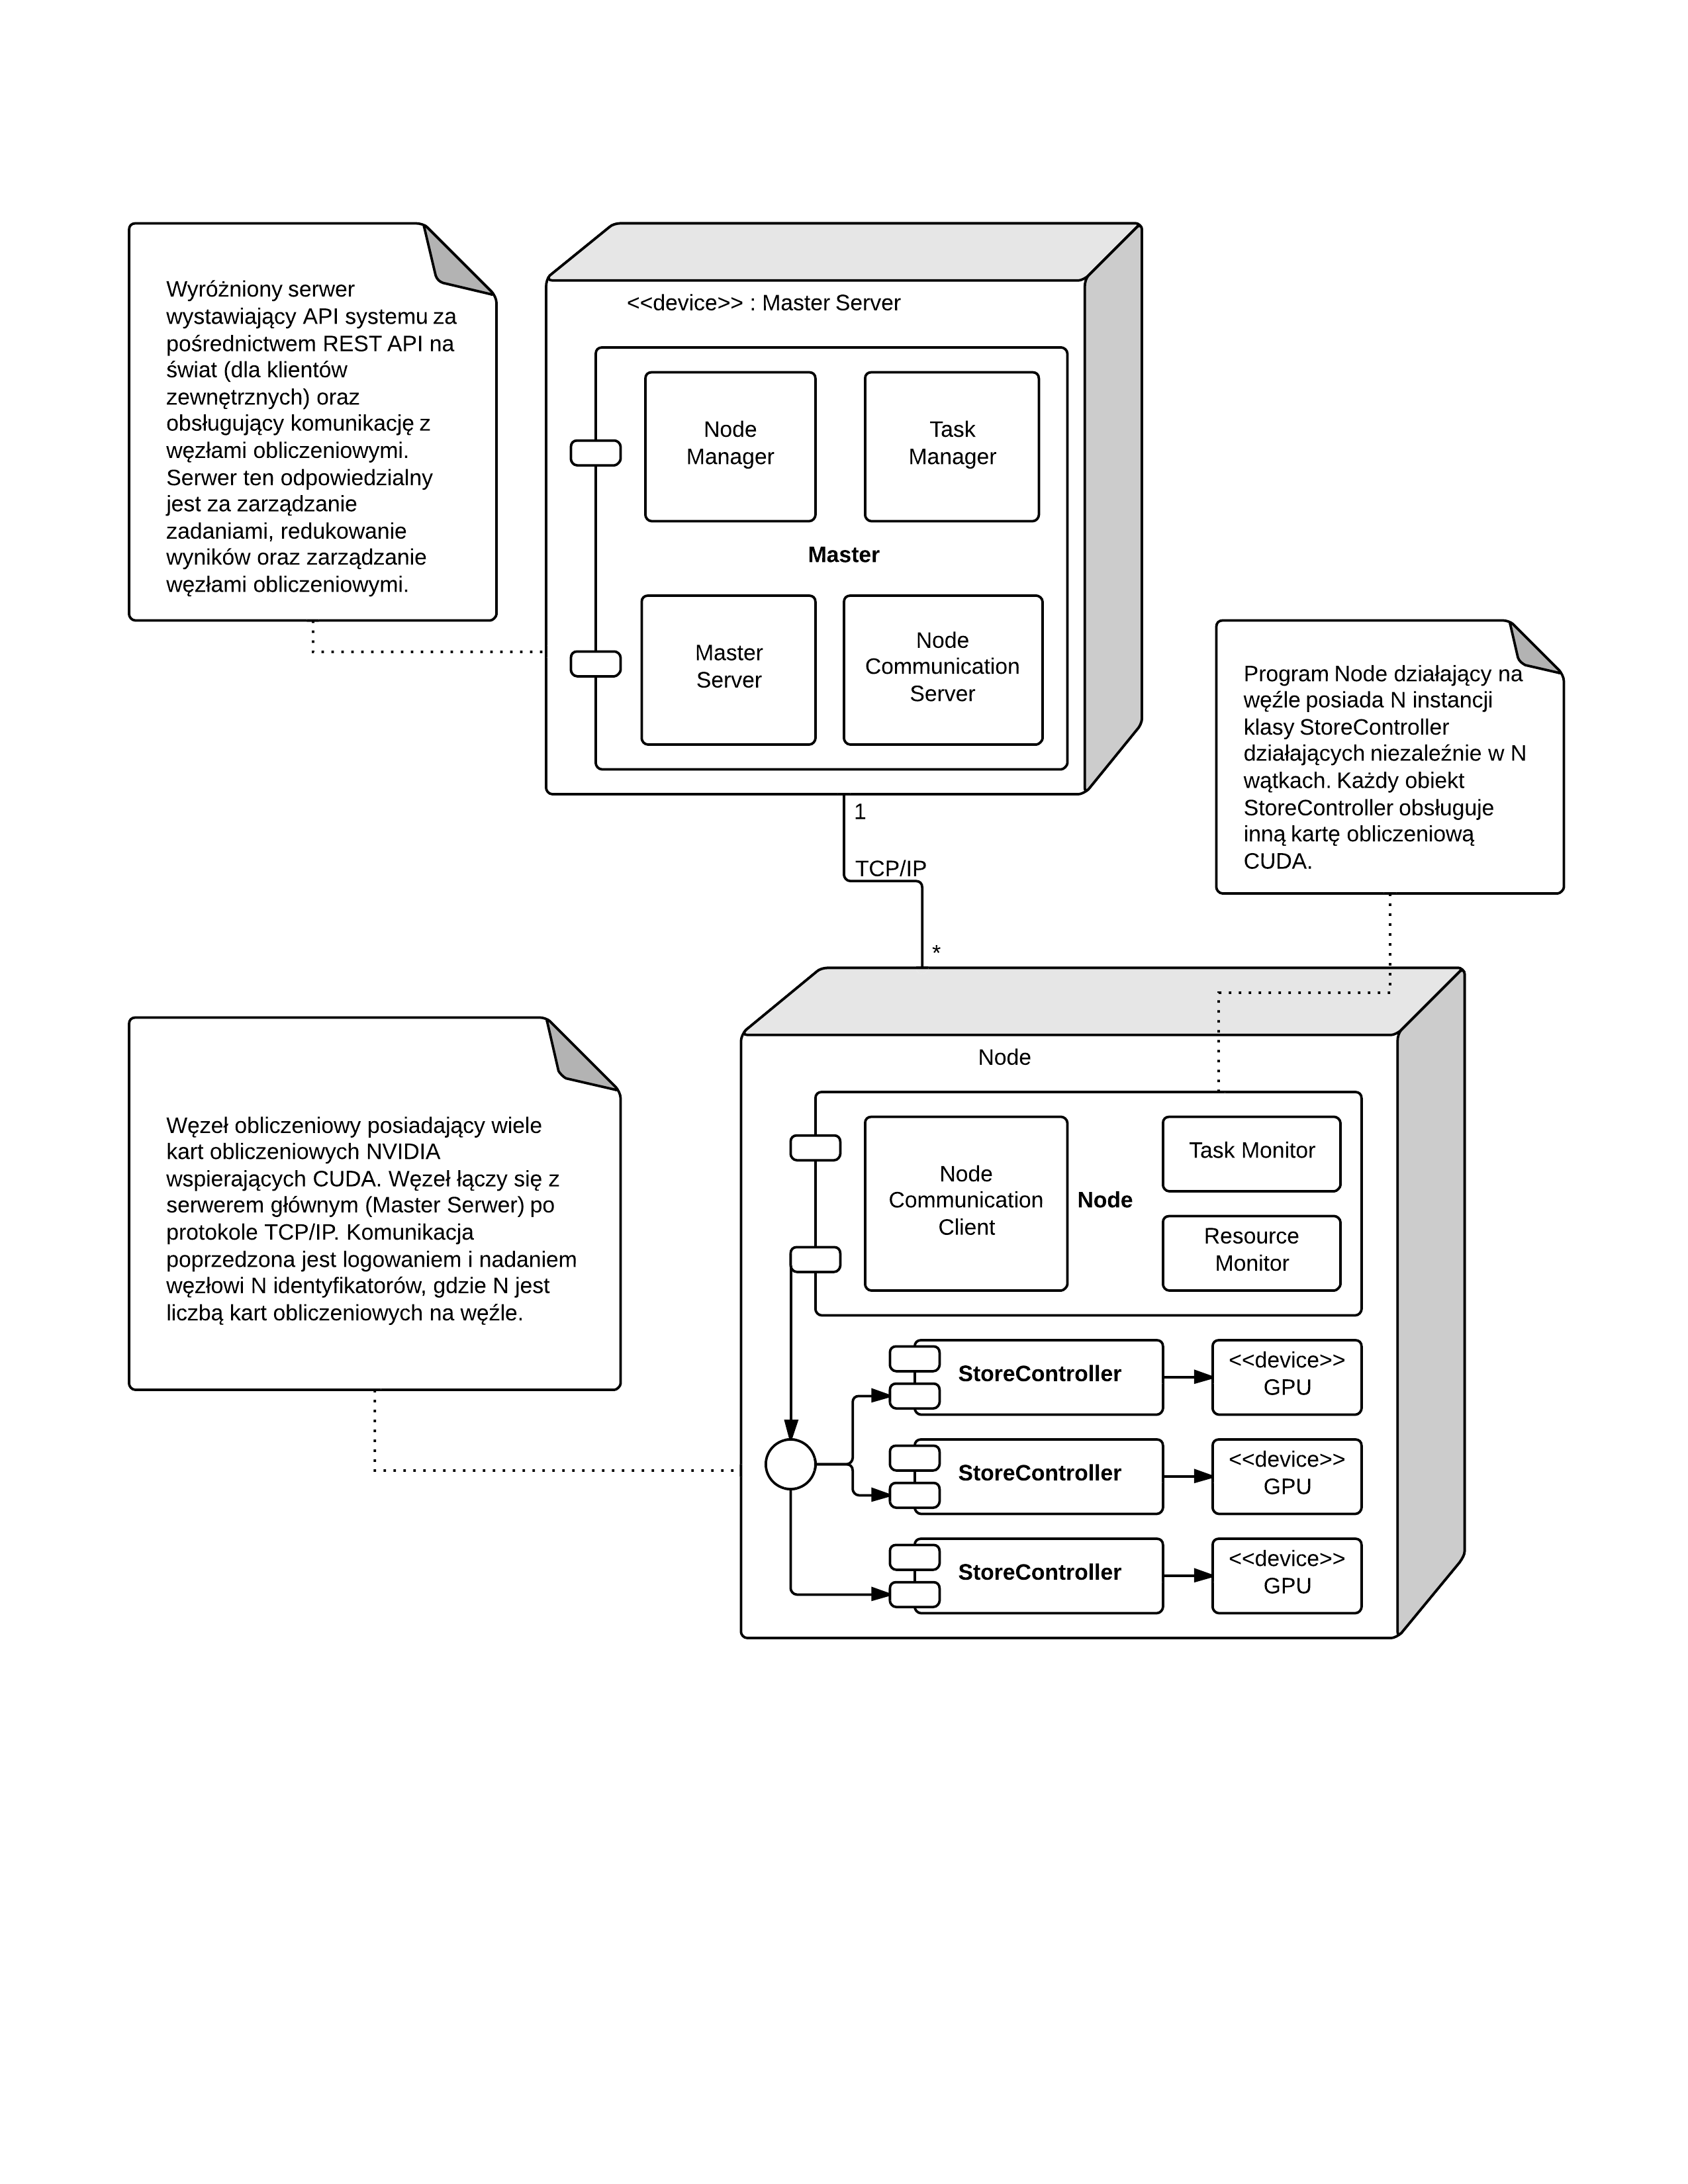
\includegraphics[width=\paperwidth]{Deployment_Diagram}}
	\end{center}
\end{figure}
\clearpage

\section{Master}

	Program głównego serwera napisany jest w języku Go\footnote{http://www.golang.org}. 
	Program korzysta między innymi z takich pakietów jak:
	\begin{description}
		 \item[log4go] do logowania
		 \item[gorest] wspomagający RESTowe API 
		 \item[gcfg] do konfiguracji.
	\end{description}		
	
	\subsection{Struktura}
		W obecnej implemntacji skupiono się na poprawnej implementacji komunikacji pomiędzy Masterem a jednym Nodem.
		Obiekty przesyłane przez sieć są serializowane binarnie i poprzedzane nagłówkiem, który zawiera informacje
		o typie i rozmiarze zadania. Kod programu podzielono na następujące pakiety
		\begin{description}
			\item[dto] Zbiór wszystkich obiektów, które są przesyłane pomiędzy poszczególnymi elementami systemu
			\item[rest] Definicja i implementacja elementów zewnętrznego, RESTowego API
			\item[node] Kod odpowiedzialny za komunikację z Node'em oraz funkcja \texttt{IOHandler}
			\item[config] Metody odpowiedzialne za ładowanie konfiguracji do globalnej struktury
			\item[constants] Stałe używane w programie
			\item[DDJ Master] Plik main programu w którym powoływane są wszystkie potrzebne serwisy
		\end{description}

	\subsection{Obecny Przepływ danych}
		Przetwarzanie zapytania RESTowego odebranego od klienta:
		\begin{enumerate}
			\item Serwer wystawiający RESTowe API otrzymuje zapytanie select lub insert, które kieruje jako request to IOHandlera
			\item Tworzone jest nowe zapytanie (Query), które jest przesyłane do Noda
			\item Jeśli zapytanie jest typu select, to przed wysłaniem do Noda, identyfikator zapytania zostanie zapisany w słowniku wraz z kanałem
			wynikowym na którym słucha API
			\item NodeSender wysyła zapytania do odpowiadającego mu węzła
		\end{enumerate}
		Przetwarzanie rezultatu zapytania odebranego od węzła:
		\begin{enumerate}
			\item NodeReceiver odbiera obiekt TaskResponse, który kieruje do IOHandlera
			\item IOHandler sprawdza identyfikator zadania i przesyła jego wynik do czekającego na odpowiedź API
			\item API przesyła wynik do klienta
		\end{enumerate}
	\subsection{Problemy}
	
	Podczas testów okazało się, że zaproponowana implementacja jest niewystarczająca ze względu na wydajność systemu. Główny ciężar procesowania
	zadań był bowiem przeniesiony na funkcję \texttt{IOHandler} co powodowało że zapytania wywoływane były de facto sekwencyjnie gdyż w tej właśnie
	funkcji odbywała się serializacja binarna i zlecenie wysłania do Node'a. Była ona również odpowiedzialna za implementację TaskManager (implementowanego
	jako słownik) i odbieranie wyników zapytań od Node'a i przesyłania ich do API. Z powyższego opisu jasno wynika, że \texttt{IOHandler} przepuszczał przez
	siebie całą komunikację i blokował wszystkie inne wątki w czasie gdy sam procesował dane. 
	
	\subsection{Nowa struktura}
	
	Jeśli system ma wspierać obsługę wielu Node'ów to wydajność Mastera musi być zdecydowanie większa. Niestety obecna struktura nie pozwala na drastyczne
	zwiększenie wydajności systemu. Poniżej prezentujemy nową (poprawioną) wersję przepływu danych.
	
		\begin{figure}[t]
			\begin{center}
				\caption{Planowany przepływ serwera głównego}
 				\makebox[\textwidth]{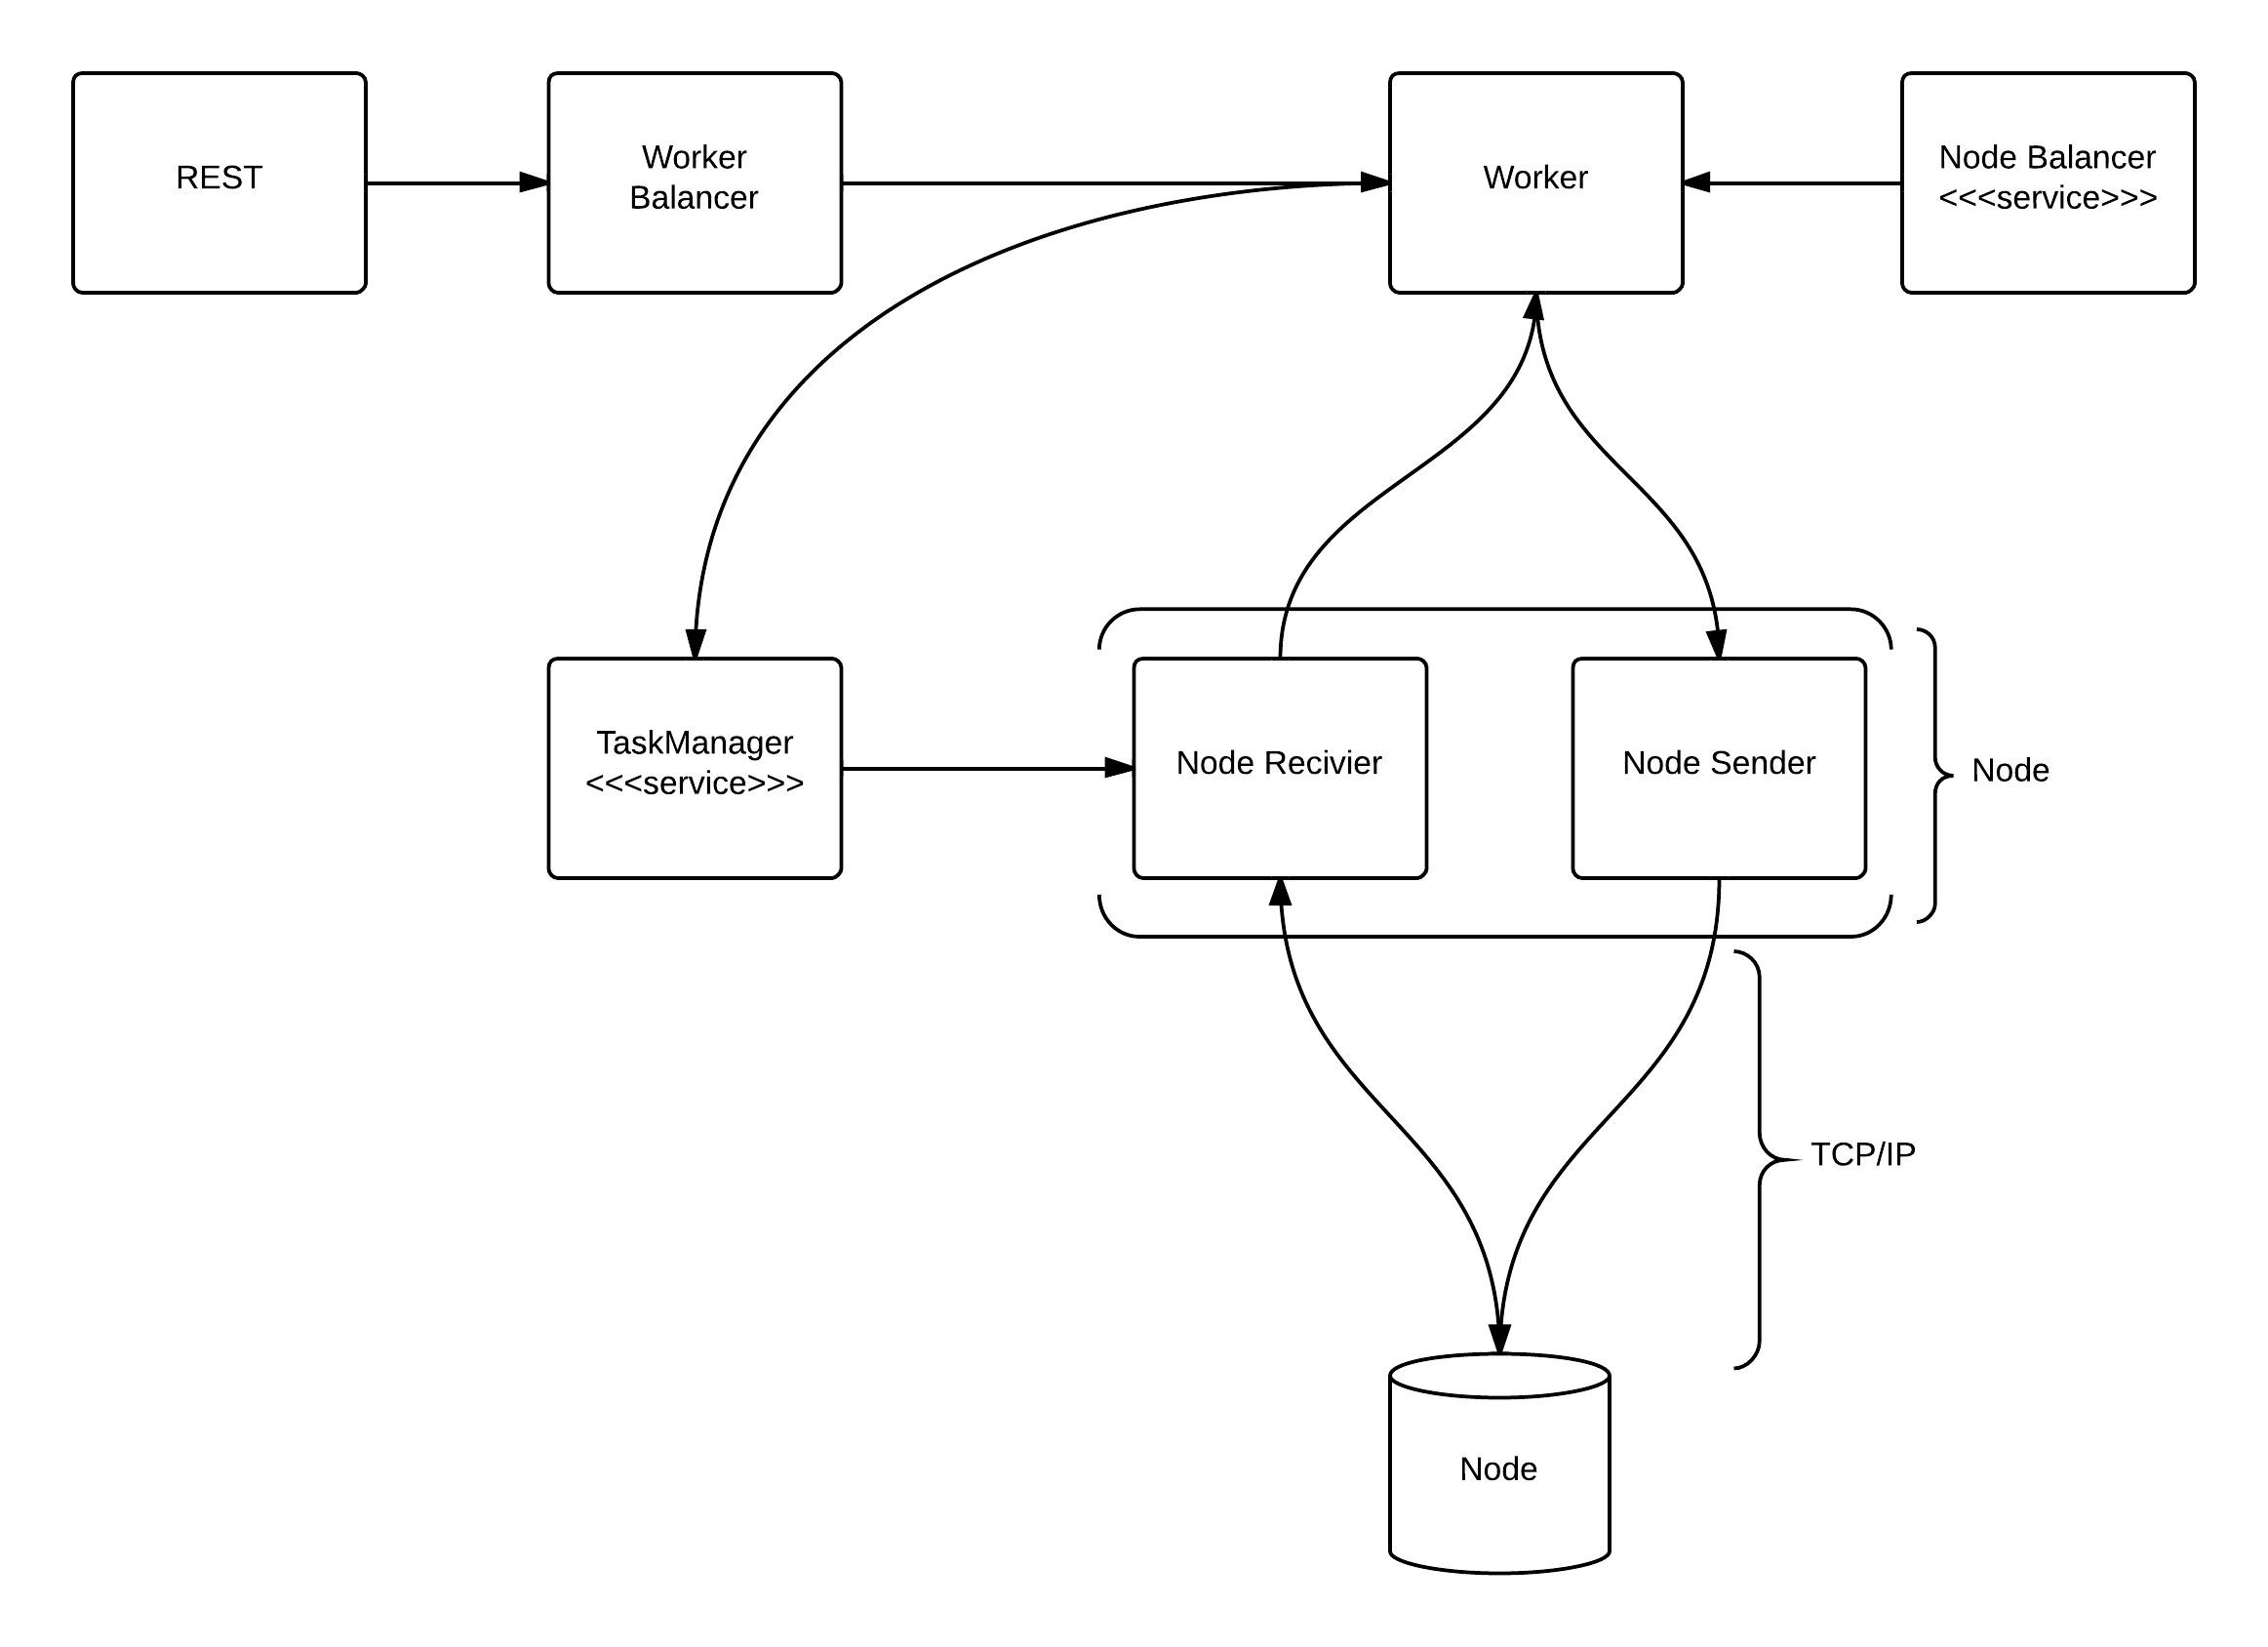
\includegraphics[width=\paperwidth]{img/Master_New_Structure}}
			\end{center}
		\end{figure}
	\clearpage
	\subsubsection{Insert}
		\begin{enumerate}
			\item Po przez API zadanie jest przyjmowane od użytkownika. Wewnątrz metody obsługującej odbywa się parsowanie JSON'a na wewnętrzne DTO i opakowanie w strukturę Task.
			\item Utworzony Task zostaje wysłany do WorkerBalancera gdzie zostaje przesłany do odpowiedniego Workera z puli.
			\item Worker odbiera Taska (jest to insert) 
			\item Worker nadaje zadaniu identyfikator z dostępnej mu puli
			\item Worker pobiera z NodeBalancera do, którego Node'a ma go wysłać. 
			\item Następnie serializuje Taska i wysyła. 
			\item Nie czeka na odpowiedź tylko od razu wysyła na kanał zwrotny że zadanie zostało przesłane do Node'a
		\end{enumerate}
	\subsubsection{Select}
		\begin{enumerate}
			\item Po przez API zadanie jest przyjmowane od użytkownika. Wewnątrz metody obsługującej odbywa się parsowanie JSONa na wewnętrzne DTO i opakowanie w strukturę Taska. 
			\item Utworzony Task zostaje wysłany do WorkerBalancera gdzie zostaje przesłany do odpowiedniego Workera z puli.
			\item Worker odbiera Taska (jest to select) 		
			\item Worker nadaje zadaniu identyfikator z dostępnej mu puli
			\item Worker pobiera z NodeBalancera listę Node'ów
			\item Worker rejestruje w TaskManagerze zadanie o nadanym wcześniej ID, które czeka na liczbę odpowiedzi różną liczbie aktywnych Node'ów
			oraz kanał zwrotny, na którym czeka na wyniki. 
			\item Worker zleca wysłanie zadania do Node'ów z listy
			\item Każdy Node obiera zadanie i procesuje je
			\item Każdy Node zwraca wynik opakowany w header z ID jest to odebrane przez NodeReceiver'a 
			\item NodeReceivier deserializuje wiadomość 
			\item NodeReceivier odczytuje z TaskManager'a, do którego Worker'a przesłać otrzymany wynik
			\item W trakcie tego sprawdzania zmniejszamy liczbę odpowiedzi, na które czeka dane zadanie
			\item Worker odebrał już wyniki od wszystkich Node'ów 
			\item Worker wykonuje redukcję otrzymanych wyników
			\item Worker wysyła zredukowany wynik na kanał, który dostał razem z zadaniem
			\item Na tym kanale słucha API i zwraca wynik działania do klienta
		\end{enumerate}
	\subsubsection{Komponenty}
		\begin{description}
		    \item[NodeBalancer] Struktura zarządzająca do którego z Node'ów przesłać dany Insert oraz przechowująca listę wszystkich Node'ów.
		    Umożliwia odświeżanie informacji o Node'ach przychodzących razem z okresowymi statusami. Na tej podstawie wybrany zostanie Node, do którego zostaną wysłane dane. 
		    \item[WorkerPool] Pula Worker'ów, z których każdy obsługuje pojedyncze zapytanie. Każdy Worker pobiera kolejne zadania z buforowanego kanale, przetwarza je, po czym zwraca wynik. 
		    Z uwagi na dużą ilość Worker'ów oraz krótki czas wykonywania zapytania, wykorzystamy listę cykliczną zamiast kolejki priorytetowej do przechowywania Worker'ów.
		    Liczba Worker'ów i rozmiar buforowanego kanału zostaną dobrane w sposób empiryczny.
		    \item[TaskManager] Słownik wszystkich trwających zadań, w którym kluczem jest identyfikator a wartością liczba oczekiwanych odpowiedzi oraz kanał obsługującego Worker'a.
		\end{description}					

\section{Node}
	Program węzła napisany jest w języku programowania C++ w wersji C++11 z użyciem bibliotek BOOST i LOG4CPLUS. Do obsługi kart 
	graficznych używane są: CUDA runtime API oraz biblioteka Thrust. Program pisany jest w oparciu o CUDA Toolkit 5.5 wraz z najnowszymi sterownikami. 
	Program używa kart graficznych o CUDA compute capability $\geq 2.0$. Do działania systemu niezbędna jest przynajmniej jedna taka karta na każdym węźle.   

	\subsection{Struktura}
		Program węzła składa się z wielu współpracujących ze sobą ,,modułów'', którym odpowiadają klasy w programie. Na każdym węźle może znajdować się
		wiele kart graficznych, które będą używane przez program jeśli spełniają wymagania. Dane będziemy wkładać na karty oraz wykonywać na nich zapytania
		niezależnie od siebie, tj. na poziomie obsługi karty nie mamy pojęcia o istnieniu innych. Architektura systemu ma na celu zapewnienie dużej 
		równoległości wykonywania zadań oraz modularności komponentów. \\
		Opis wybranych elementów struktury:
		\begin{itemize}
			\item Node - ,,Korzeń'' całego programu dla węzła. Stworzenie instancji tej klasy spowoduje rozpoczęcie działania węzła. \\ \\
				Funkcjonalność: 
				\begin{itemize}
					\item Odpowiada za uruchomienie i zatrzymanie systemu, tworzy instancję klasy StoreController dla każdej odpowiedniej karty
						graficznej, którą dany StoreController będzie obsługiwał.
					\item Przyjmuje zadania przychodzące od Mastera i zleca je odpowiednim StoreControllerom
					\item W ramach tej klasy działa wątek zbierający ukończone zadania i wysyłający ich rezultaty do Mastera
				\end{itemize}
			\item Store Controller - odpowiada za obsługę jednej karty graficznej o podanym numerze. \\ \\
				Funkcjonalność: 
				\begin{itemize}
					\item Alokuje główną tablicę na dane na karcie graficznej, w której przechowywane będą dane
					\item Wykonuje zadania przydzielone mu przez Node'a
					\item Zarządza strukturami do wykonywania zadań: wieloma obiektami Store Buffer (jeden dla każdej metryki) oraz obiektem Query Monitor
				\end{itemize}
			\item Store Buffer - obsługuje wpływające rekordy z jedną metryką \\ \\
				Funkcjonalność: 
				\begin{itemize}
					\item Podwójnie buforuje przychodzące dane
					\item Zamienia bufory jeśli główny się napełnił i zleca załadowanie przechowywanych w buforze danych na GPU
					\item Składuje informacje o położeniu danych w pamięci GPU w B+ drzewie za pomocą obiektu BTreeMonitor
				\end{itemize}
			\item Network Client (Node Communication Client) - odpowiada za komunikację z Masterem \\ \\
				Funkcjonalność: 
				\begin{itemize}
					\item Loguje węzeł do serwera głównego
					\item Odbiera zlecenia wykonania zadań od Mastera
					\item Wysyła rezultat wykonanego zadania do Mastera
				\end{itemize}
			\item Node Controller (Resource Controller) - nadzoruje wykorzystanie zasobów na węźle i przesyła ja do Mastera \\ \\
				Funkcjonalność: 
				\begin{itemize}
					\item Pobiera dane o wykorzystaniu CPU, RAM, GPU
					\item Pobiera dane o ilości wolnego i zajętego miejsca w głównej tablicy danych na GPU
					\item Wysyła statystyki do Mastera
				\end{itemize}
			\item Moduły nazywane X Monitor mają za zadanie zarządzanie dostępem do zasobów X oraz synchronizację wątków
		\end{itemize}
		\begin{figure}[t]
			\begin{center}
				\caption{Struktura węzła}
 				\makebox[\textwidth]{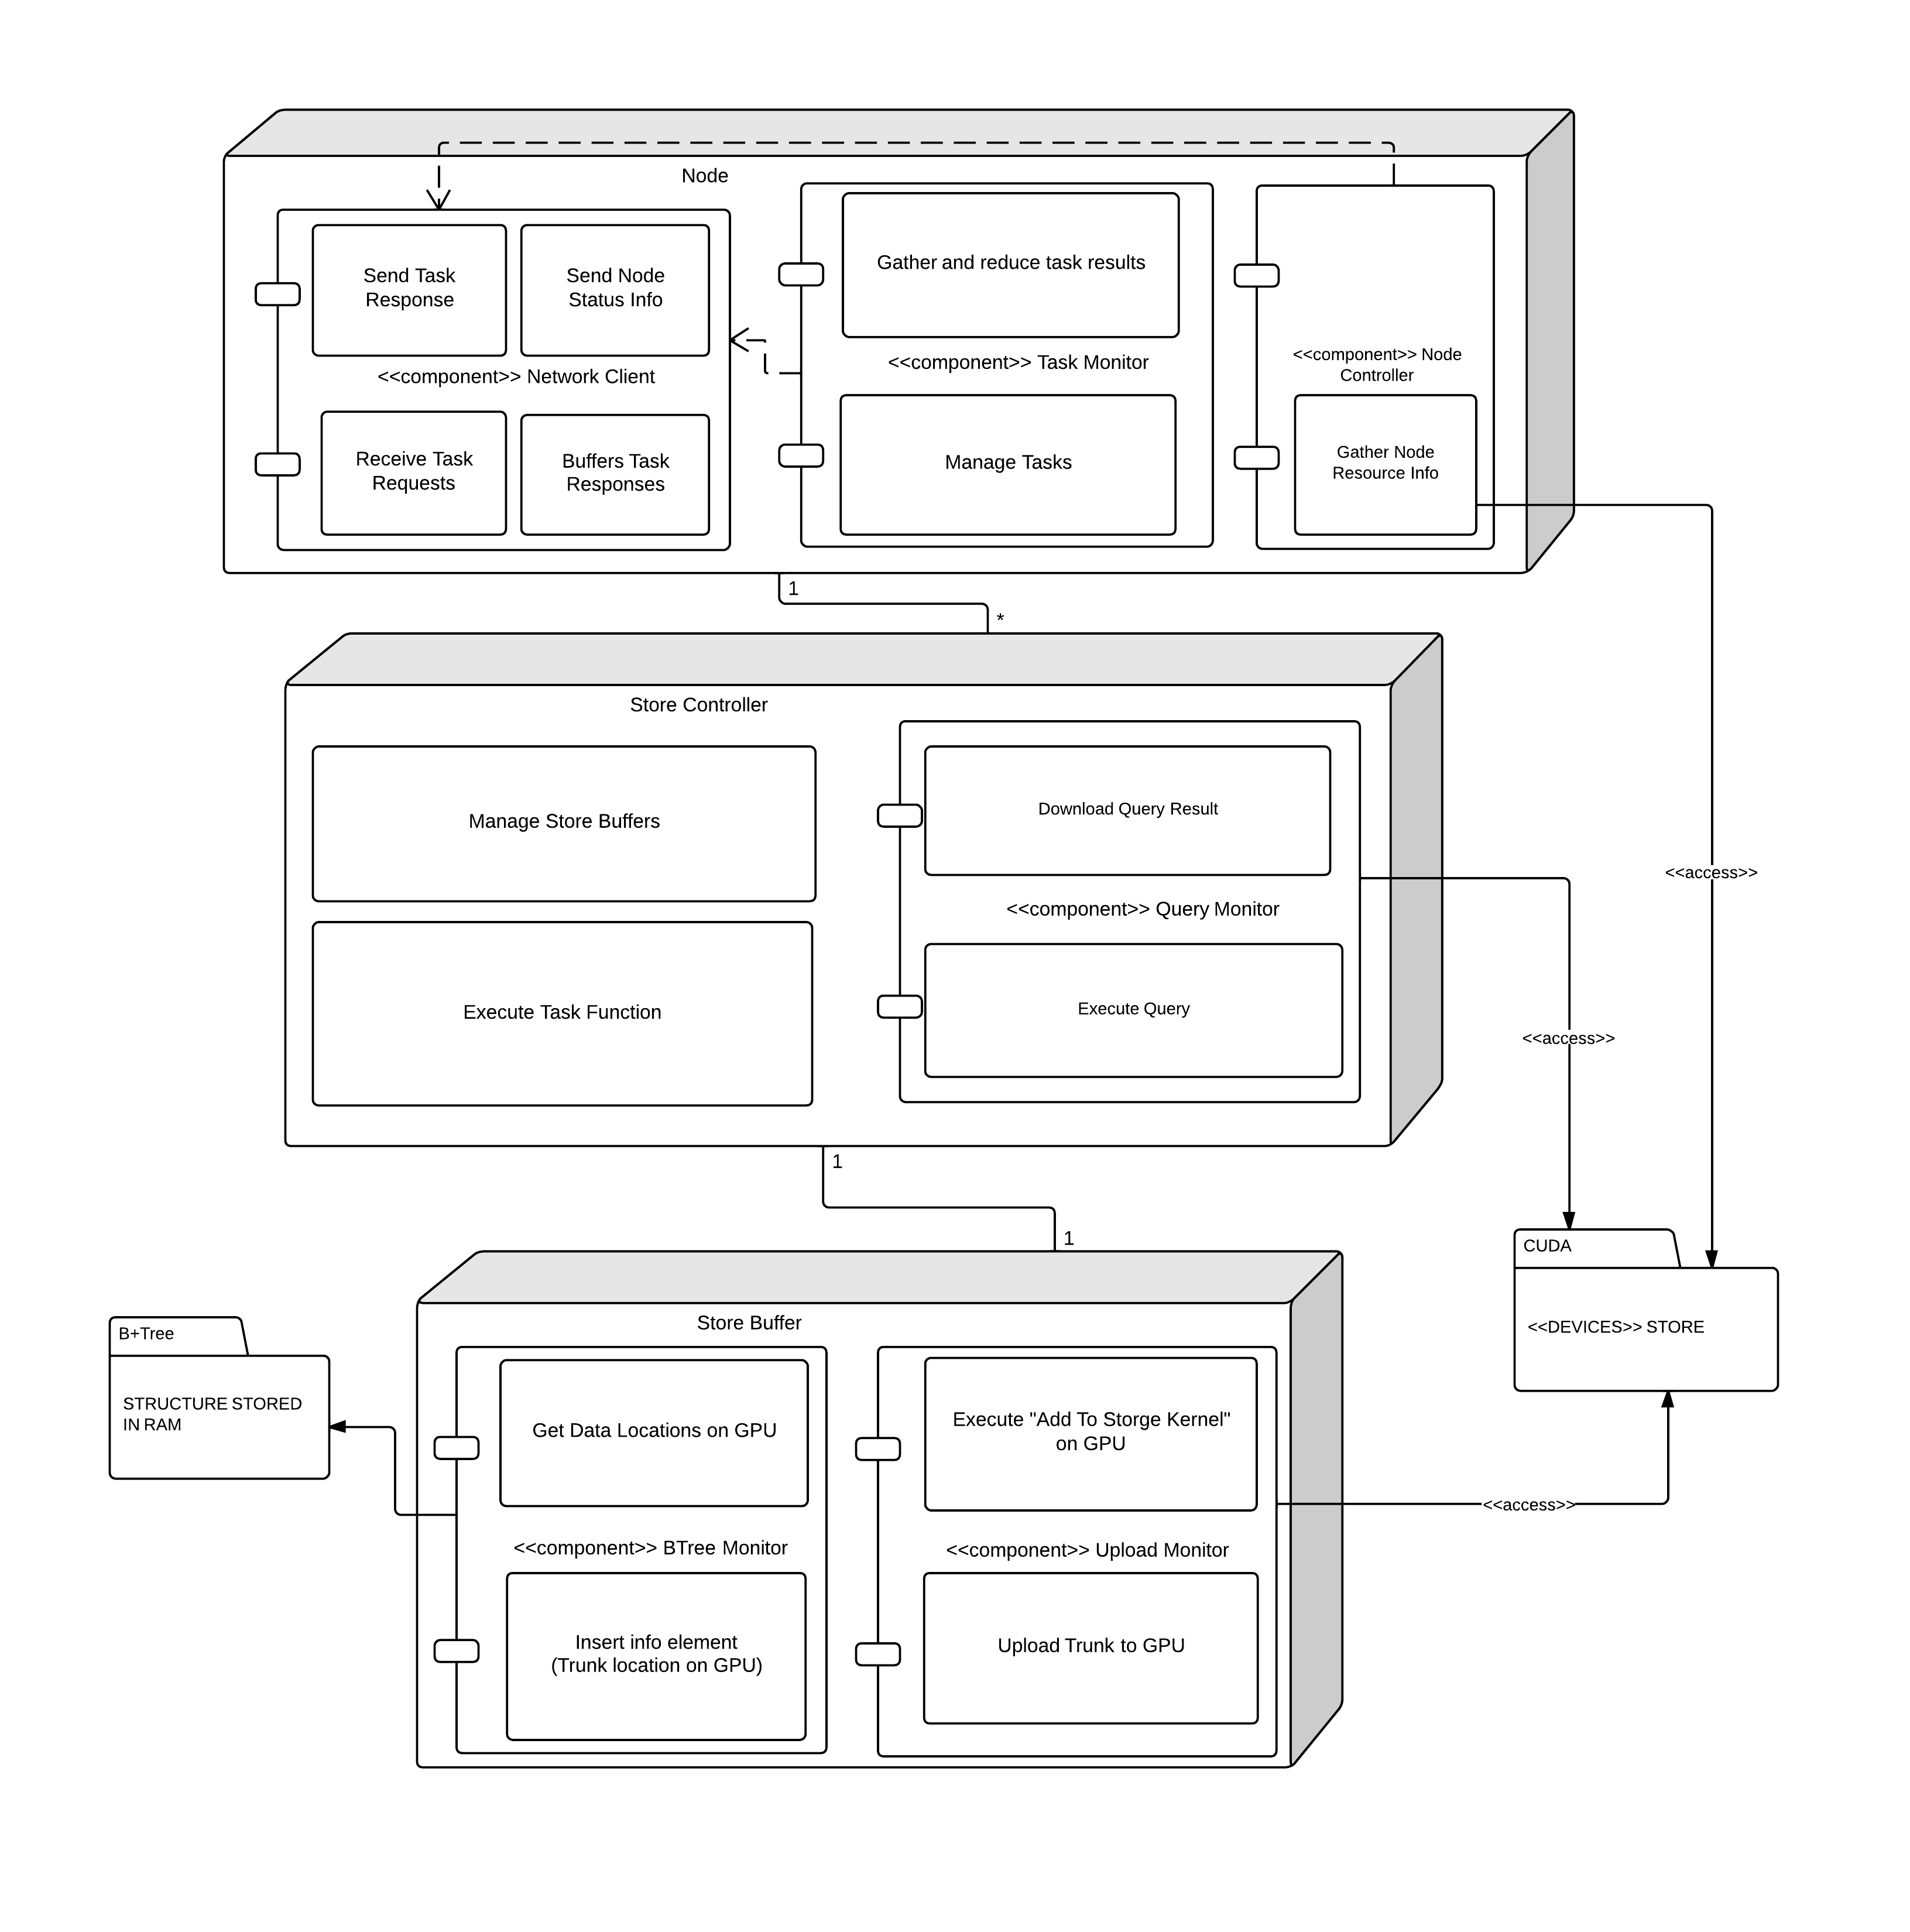
\includegraphics[width=\paperwidth]{Component_Node}}
			\end{center}
		\end{figure}
		\clearpage

	\subsection{Przepływ danych}
		Przepływ danych w węźle przy wykonywaniu operacji Insert (wkładania danych do bazy danych):
		\begin{enumerate}
			\item Node Communication Client otrzymuje TaskRequest od Mastera zawierający typ zadania (INSERT), identyfikator mówiący 
				na której karcie dane mają być umieszczone oraz element do załadowania do bazy.
			\item TaskRequest poprzez sygnał (boost.Signals) przekazywany jest do Node'a, który przekazuje TaskRequest do Task Monitora. Ten tworzy 
				obiekt zadania (StoreTask)
			\item StoreTask przekazywany jest po identyfikatorze do odpowiedniego StoreControllera odpowiadającego za kartę, w której umieszczone mają być dane
			\item StoreController wykonuje zadanie przekazując element do załadowania do bazy do bufora (StoreBuffer)
			\item StoreController wykonuje na zadaniu SetResult z pozytywnym wynikiem. Wtedy zadanie może być zakończone i usunięte
			\item Jeśli bufor w danym obiekcie StoreBuffer stanie się pełny bufor zostaje zamieniony na pusty, a pełny trafia do Upload Monitora, który załaduje dane na GPU
			\item Po udanym załadowaniu danych na GPU informacje o położeniu danych na karcie zwrócone przez UploadMonitor w postaci struktury infoElement, która przekazywana jest do
				BTree Monitora w celu umieszczenia jej w B+Drzewie 
			\item Dopiero po ukończeniu tych wszystkich kroków można uznać daną za włożoną do bazy danych
		\end{enumerate}
		Przepływ danych w węźle przy wykonywaniu zapytania typu Select (pobieranie danych z bazy danych):
		\begin{enumerate}
			\item Node Communication Client otrzymuje TaskRequest od Mastera zawierający typ zadania (SELECT) oraz dane do zapytania (np. filtry)
			\item TaskRequest poprzez sygnał (boost.Signals) przekazywany jest do Node'a, który przekazuje TaskRequest do Task Monitora. Ten tworzy 
				obiekt zadania (StoreTask)
			\item StoreTask przekazywany jest do wszystkich StoreController'ów
			\item Store Controller przekazuje do swojego wątku odpowiedzialnego za zapytania zadanie do wykonania (ten wątek nazywać będziemy queryThread). 
			\item queryThread prosi odpowiednie obiekty StoreBuffer'ów o informacje na temat położenia danych w pamięci GPU i dostaje je pobrane z B+drzew w postaci listy infoElement'ów
			\item queryThread tworzy obiekt QueryRequest na podstawie zapytania i infoElement'ów i przekazuje go do Query Monitora, który wykonuje operację query i zwraca mu QueryResult. 
			\item Wątek wykonujący zapytania na podstawie QueryResult wywołuje operację SetResult na zadaniu, które może być następnie uznane za wykonane
			\item Wątek w obiekcie Node odpowiedzialny za zarządzanie ukończonymi zadaniami otrzyma takie zadanie z Task Monitora po wykonaniu na nim funkcji PopCompletedTasks
				i może pobrać wynik danego zadania oraz wysłać go do Mastera 
		\end{enumerate}
		\begin{figure}[t]
			\begin{center}
				\caption{Przepływ danych dla węzła}
 				\makebox[\textwidth]{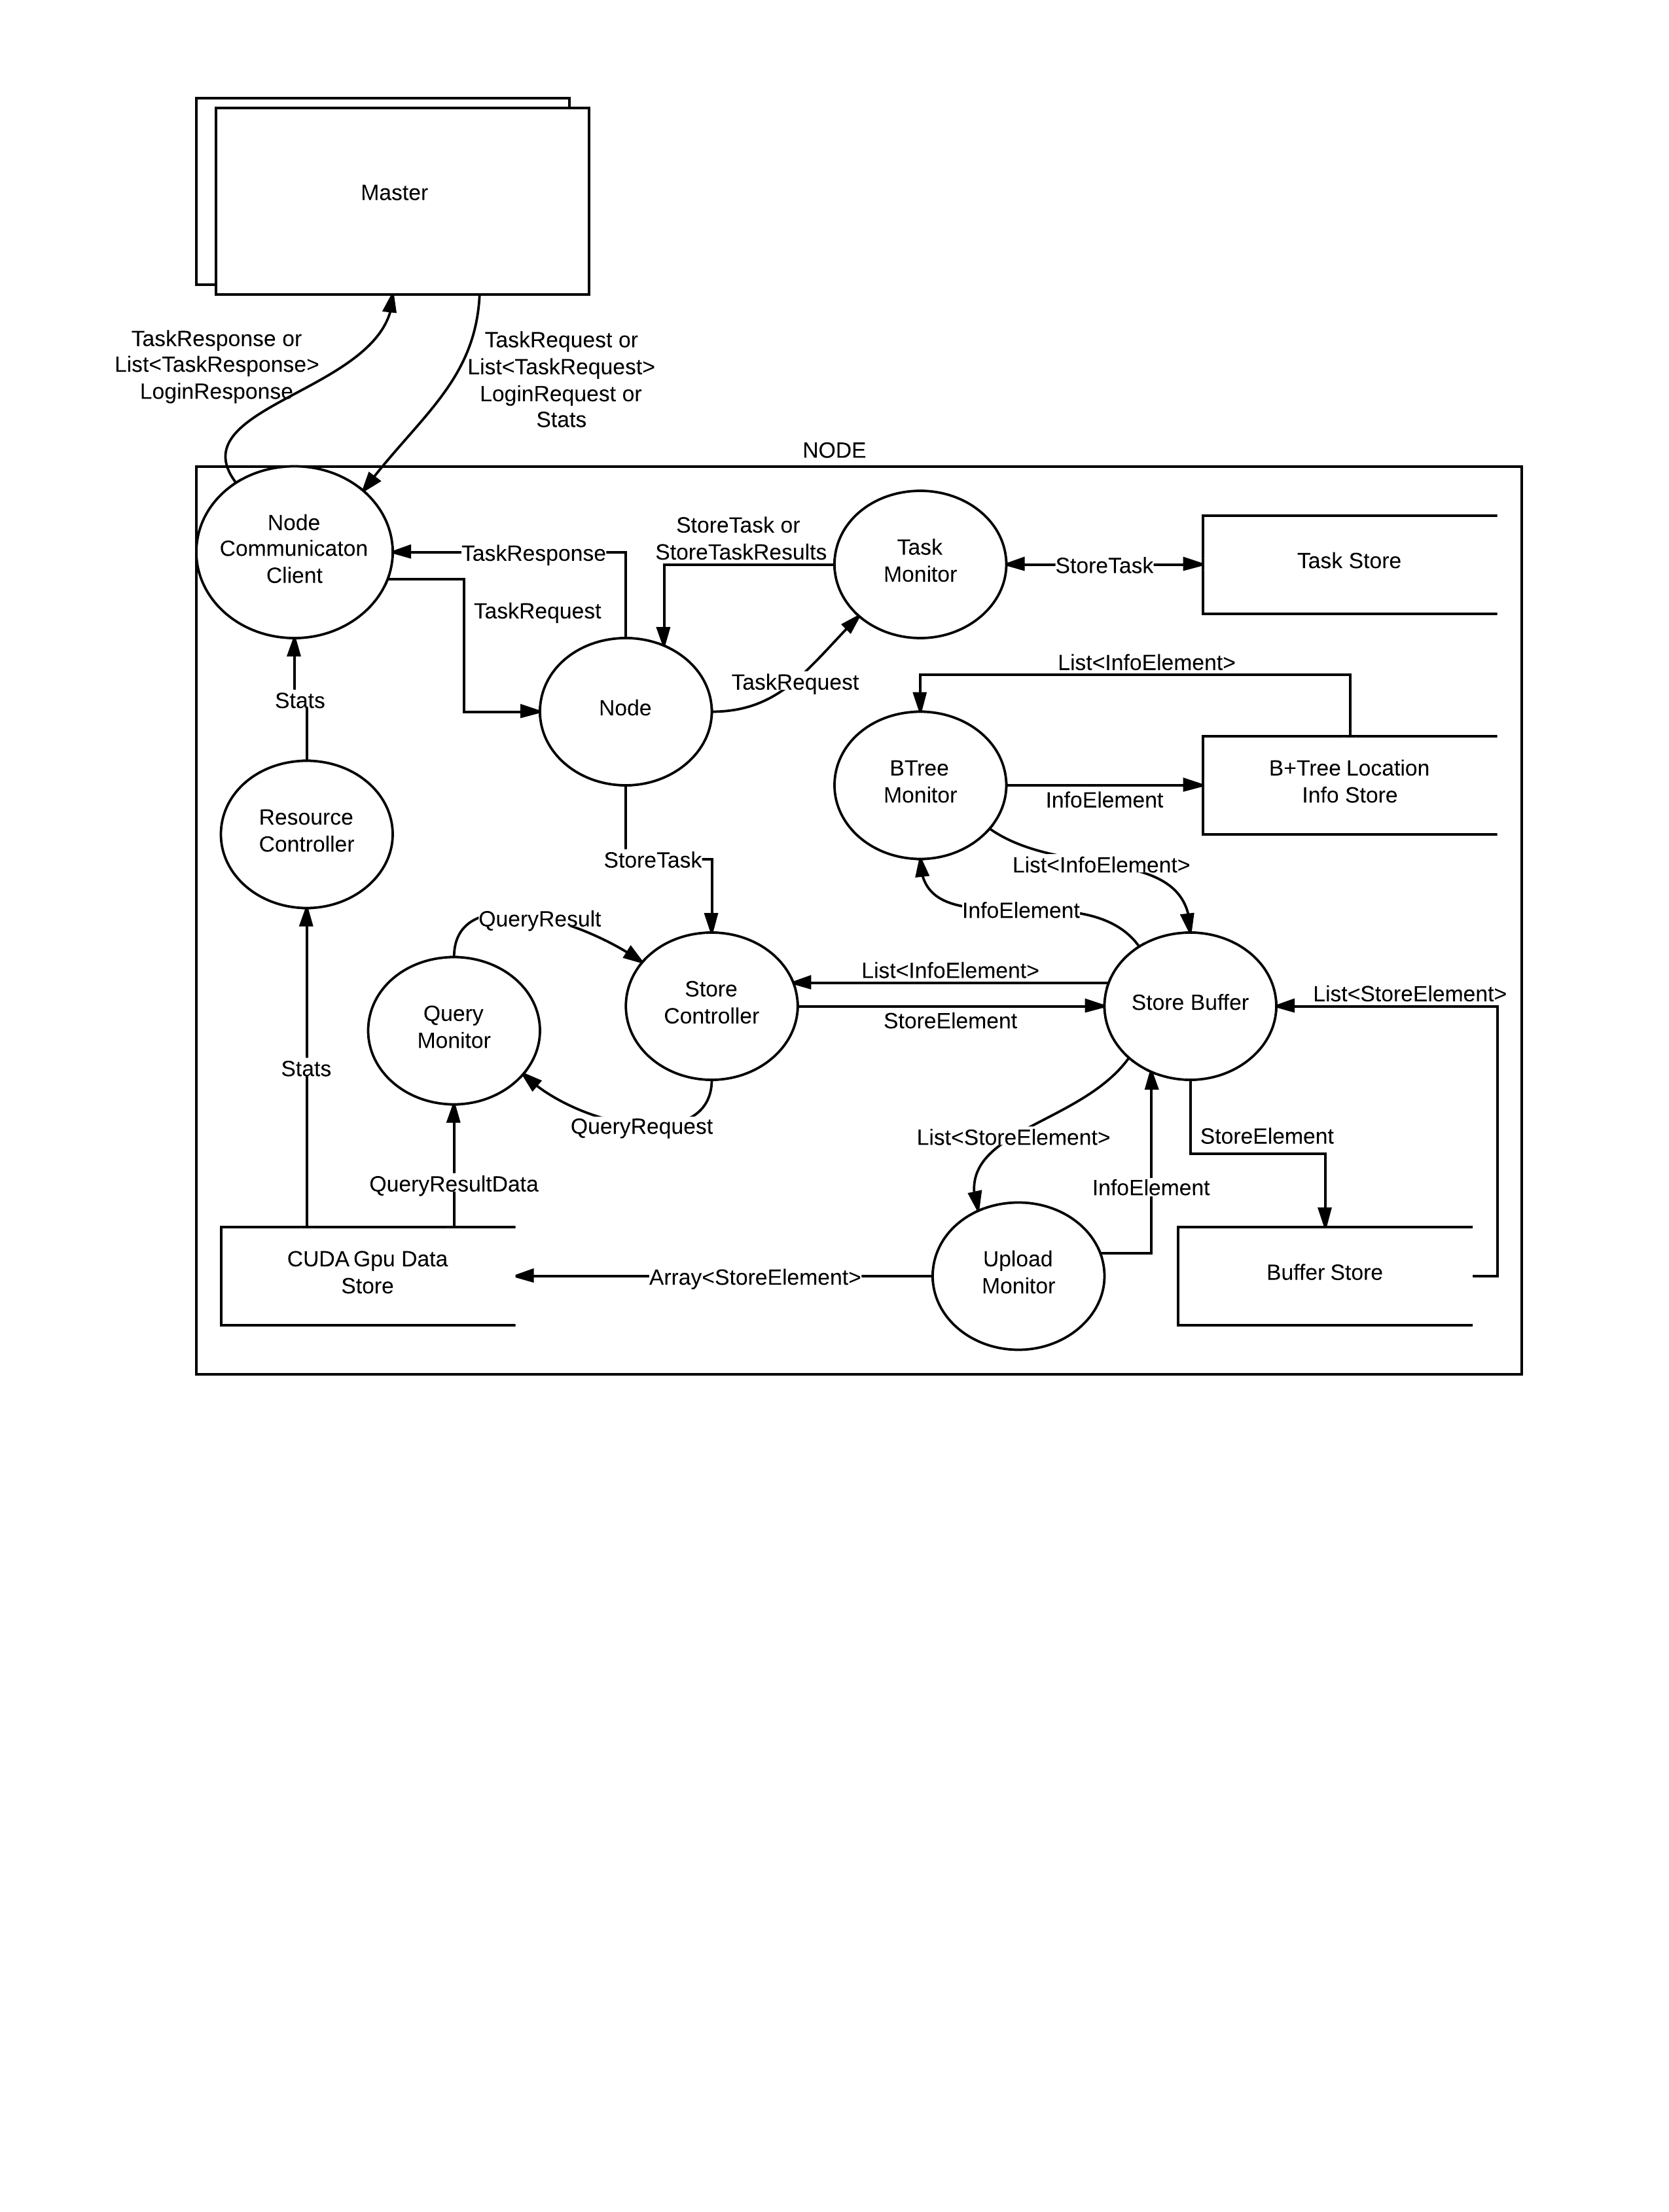
\includegraphics[width=\paperwidth]{DataFlow_Node}}
			\end{center}
		\end{figure}
		\clearpage

	\subsection{System od strony GPU}
		W tym przypadku również rozpatrywać będziemy działanie systemu osobno pod względem wrzucania danych do bazy i pod względem zapytań typu Select. \\ \\
		Insert: \\
		\begin{enumerate}
			\item Upload Monitor kopiuje bufor otrzymany od StoreBuffera do bufora po stronie GPU. Dopiero po tym kroku bufor w StoreBufferze może być ponownie zamieniony.
			\item Następnie Upload Monitor wywołuje Compressor aby ten skompresował bufor znajdujący się na GPU i zwrócił mu wskaźnik na skompresowane dane.
			\item Skompresowane dane są kopiowane w odpowiednie miejsce w głównej tablicy GPU po czym informacja o położeniu tych danych zwracana jest w postaci 
				obiektu infoElement
		\end{enumerate}
		Select: \\
		\begin{enumerate}
			\item Query Monitor po otrzymaniu QueryRequest od Store Controllera wywołuje Compressor aby ten rozkompresował dane, na które wskazują struktury infoElement zawarte w zapytaniu
			\item Następnie QueryMonitor wywołuje odpowiedni dla danego zapytania kernel wykonujący się na GPU przekazując mu wskaźnik do rozkompresowanych danych 
			\item Dane mogą być odpowiednio filtrowane w zależności od zapytania przez funkcję wywołaną z kernela
			\item Wskaźnik na rezultat zapytania zwracany jest do QueryMonitora, który pobiera dane z GPU i przesyła z powrotem do StoreControllera
		\end{enumerate}
		\begin{figure}[t]
			\begin{center}
				\caption{Działanie bazy od strony karty graficznej}
 				\makebox[\textwidth]{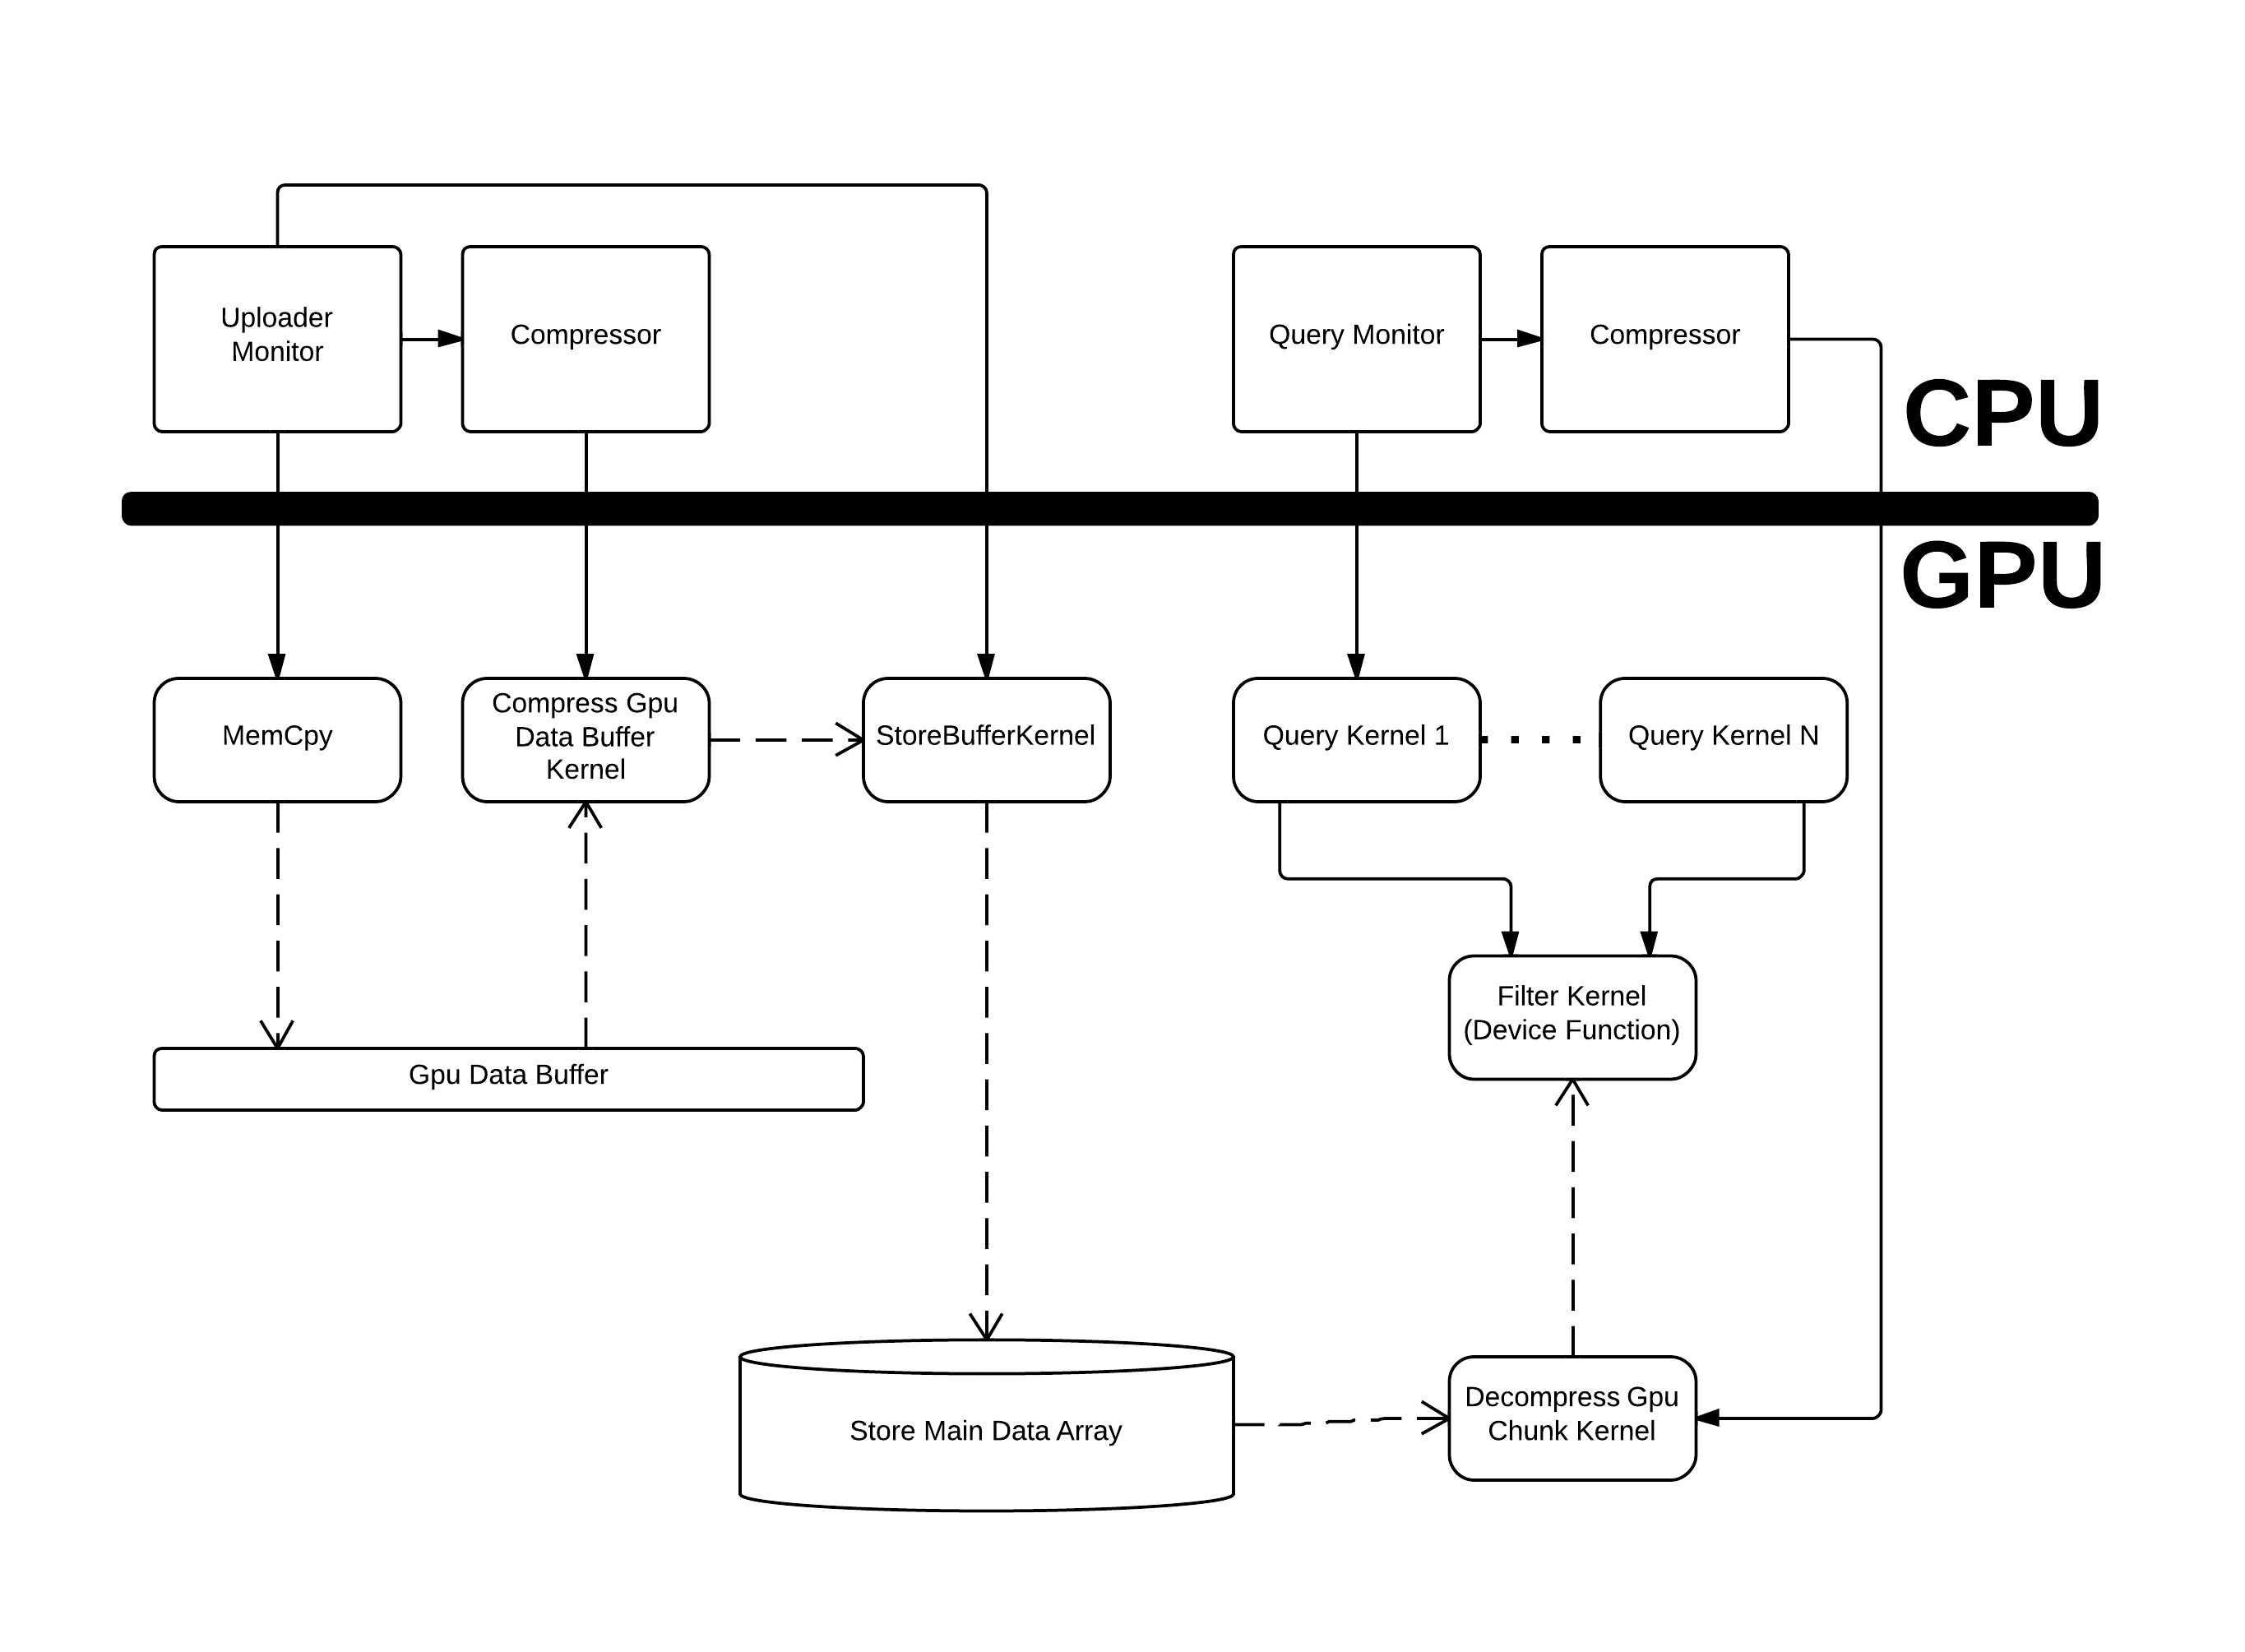
\includegraphics[width=\paperwidth]{Cuda_Store_Structure}}
			\end{center}
		\end{figure}
		\clearpage

	\subsection{Strumienie CUDA dla operacji Insert}
		Do zarządzania strumieniami CUDA zarówno dla operacji Insert jak i Select wydzielona została klasa CudaController. Zarządzanie strumieniami zostało zaimplementowane tak aby:
		\begin{itemize}
			\item Liczba strumieni przeznaczona dla operacji Insert jak również Select była łatwo konfigurowalna. 
			\item Dla konkretnego bufora operacje kopiowania bufora na GPU oraz późniejszej kompresji załadowanego bufora wykonywały się w jednym strumieniu
			\item Dla operacji kopiowania skompresowanych buforów do głównej tabeli GPU wyróżniony był jeden strumień i wszystkie takie kopiowania były wykonywane tylko w nim.
		\end{itemize}
		\begin{figure}[t]
			\begin{center}
				\caption{Zarządzanie strumieniami CUDA przy operacji Insert}
 				\makebox[\textwidth]{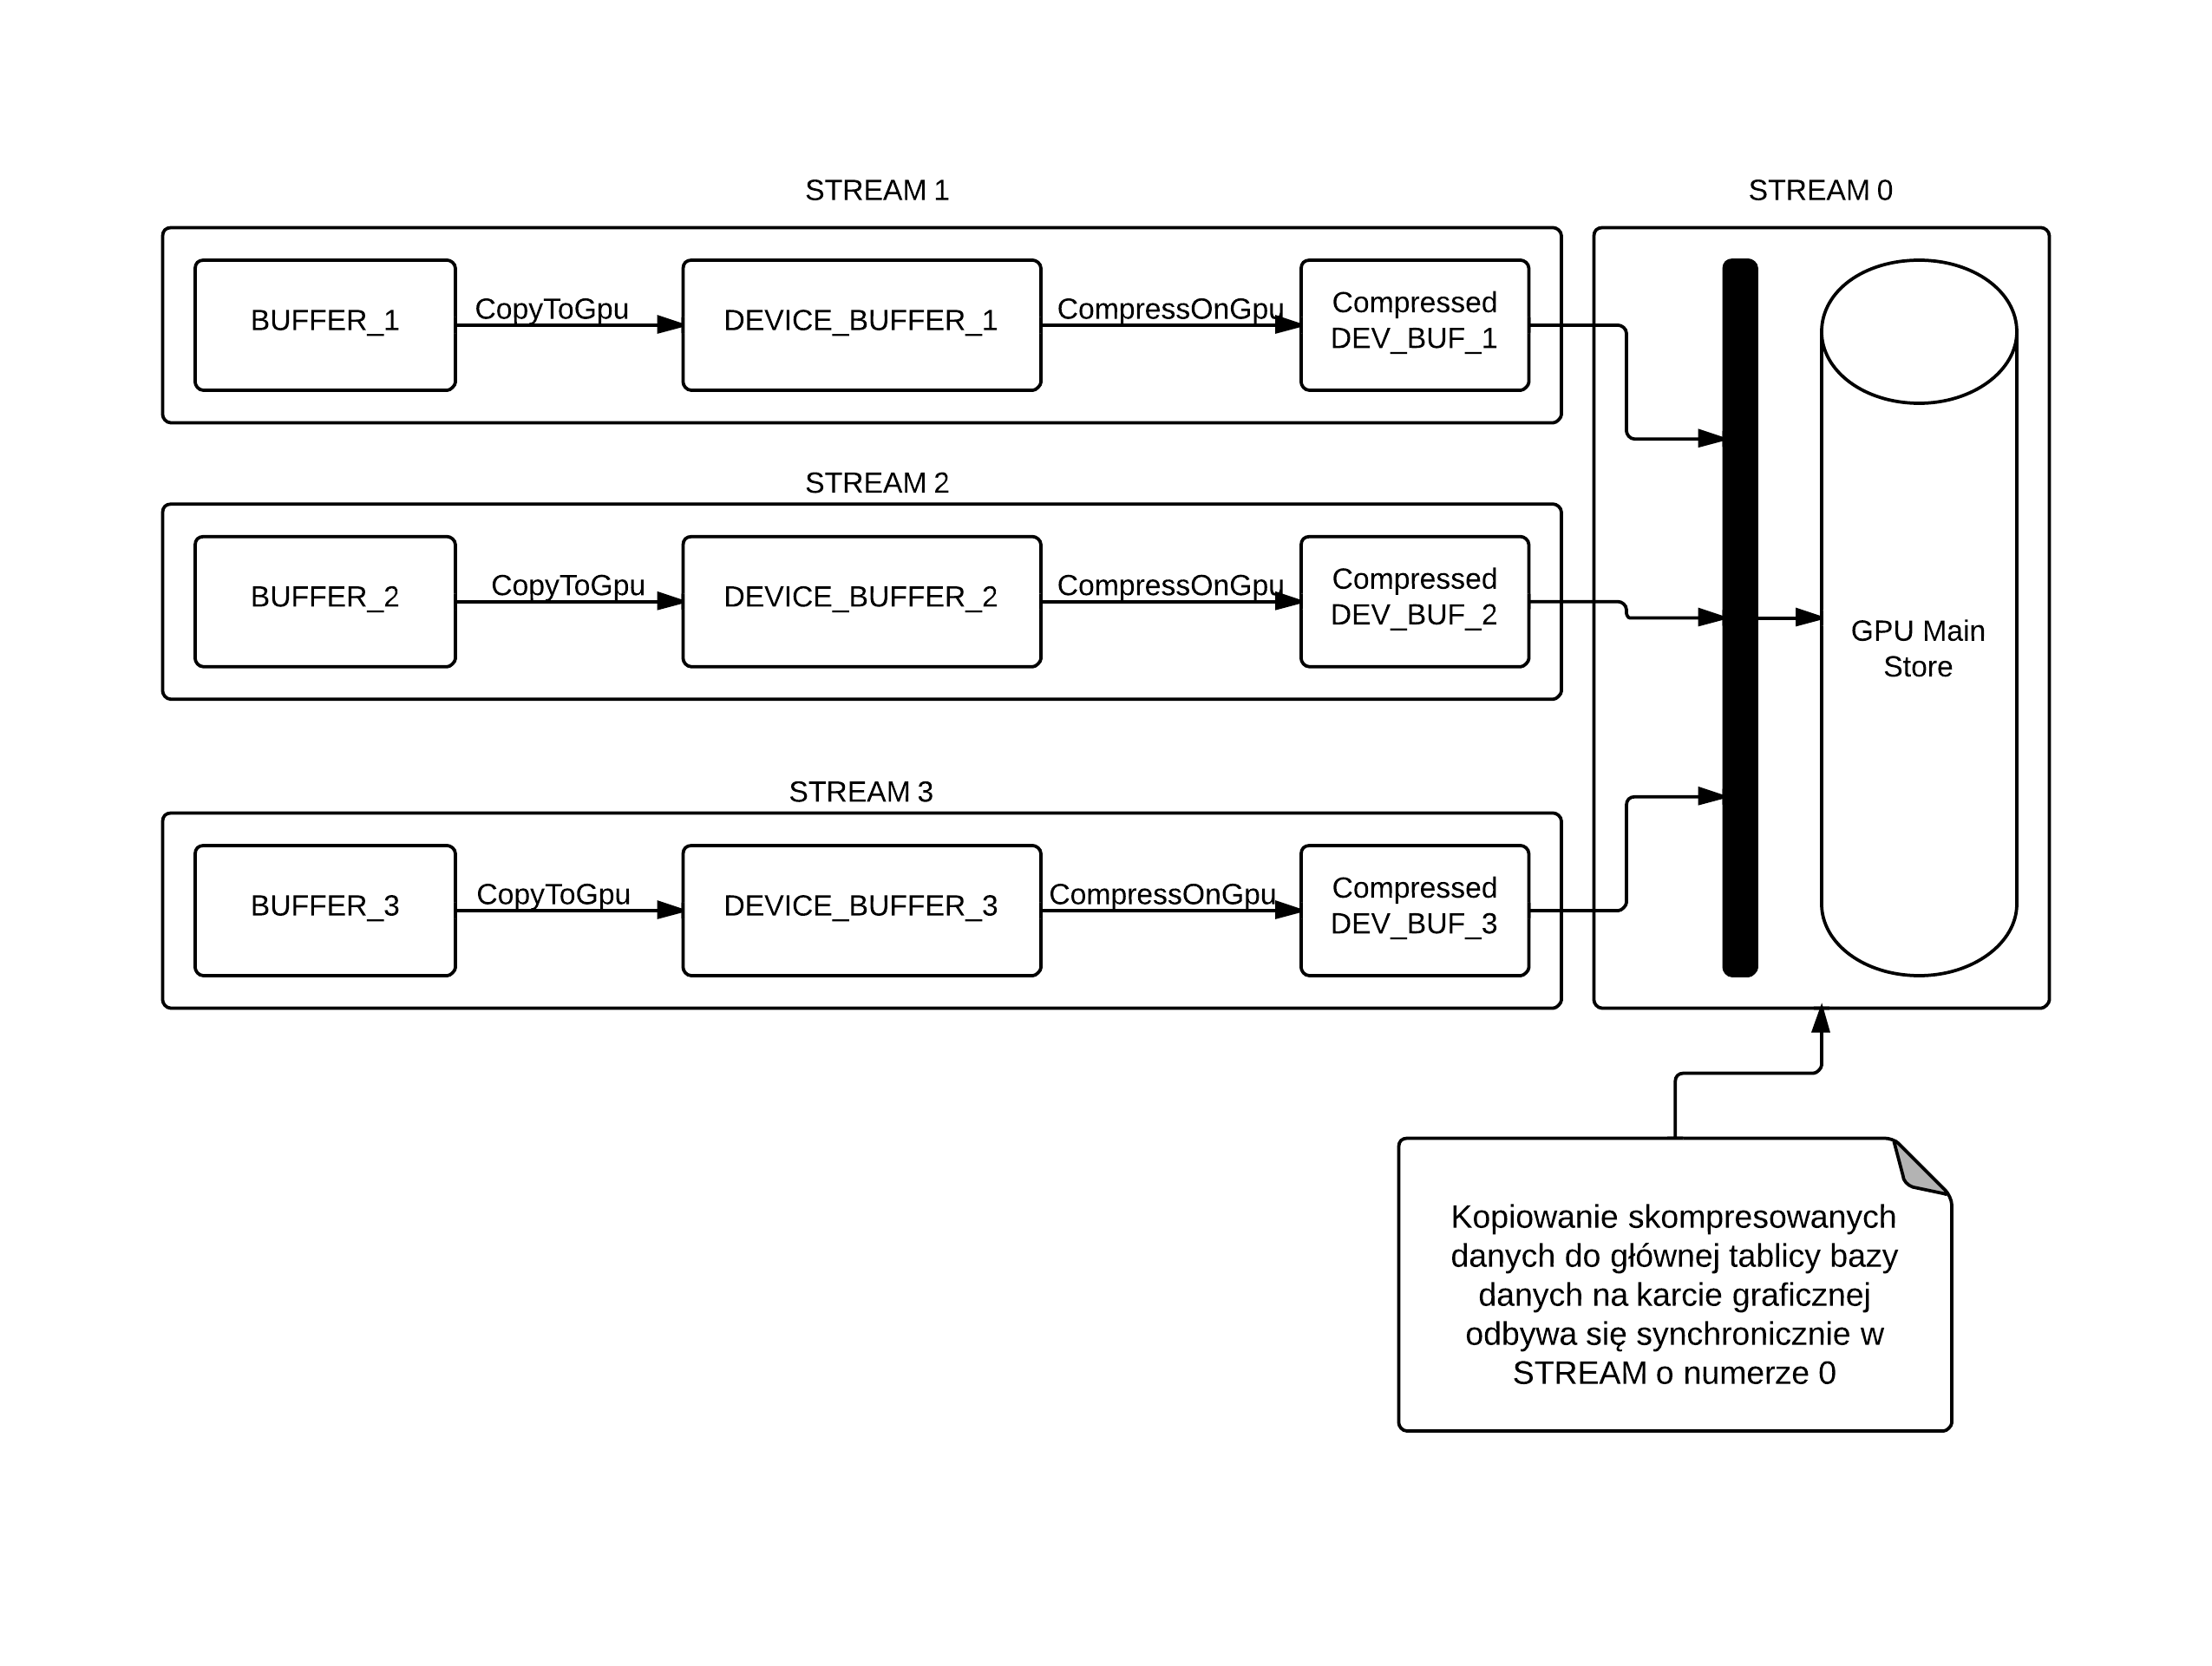
\includegraphics[width=0.9\textwidth, height=0.7\textwidth]{Cuda_Upload_Streams}}
			\end{center}
		\end{figure}
		\clearpage

\section{Map-Reduce}
Zaletą systemu będzie implementacja uproszczonego modelu programowania Map-Reduce, jako że jest to rozproszona baza danych.

\begin{itemize}
	\item Każdy z węzłów wyszukuje w swojej bazie odpowiednie fragmenty danych i wykonuje na nich operację Map tj. filtruje dane pod kątem pewnych 
		kryteriów, przy czym jeśli ilość dostępnej pamięci na karcie na to pozwala wykonywać się będzie tylko jedna operacja Map per węzeł dla danego zapytania.
		Dane uzyskane poprzez wykonanie operacji map są parami klucz-wartość, gdzie kluczem jest id danego zadania, a wartościami wyniki zapytania. Wyniki
		operacji Map z każdego węzła przekazywane są do Mastera w celu wykonania na nich operacji Reduce, która wszystkie agreguje dane zwrócone dla konkretnego zadania. 
		\begin{figure}[t]
			\begin{center}
				\caption{Ogólny schemat Map-Reduce w systemie}
 				\makebox[\textwidth]{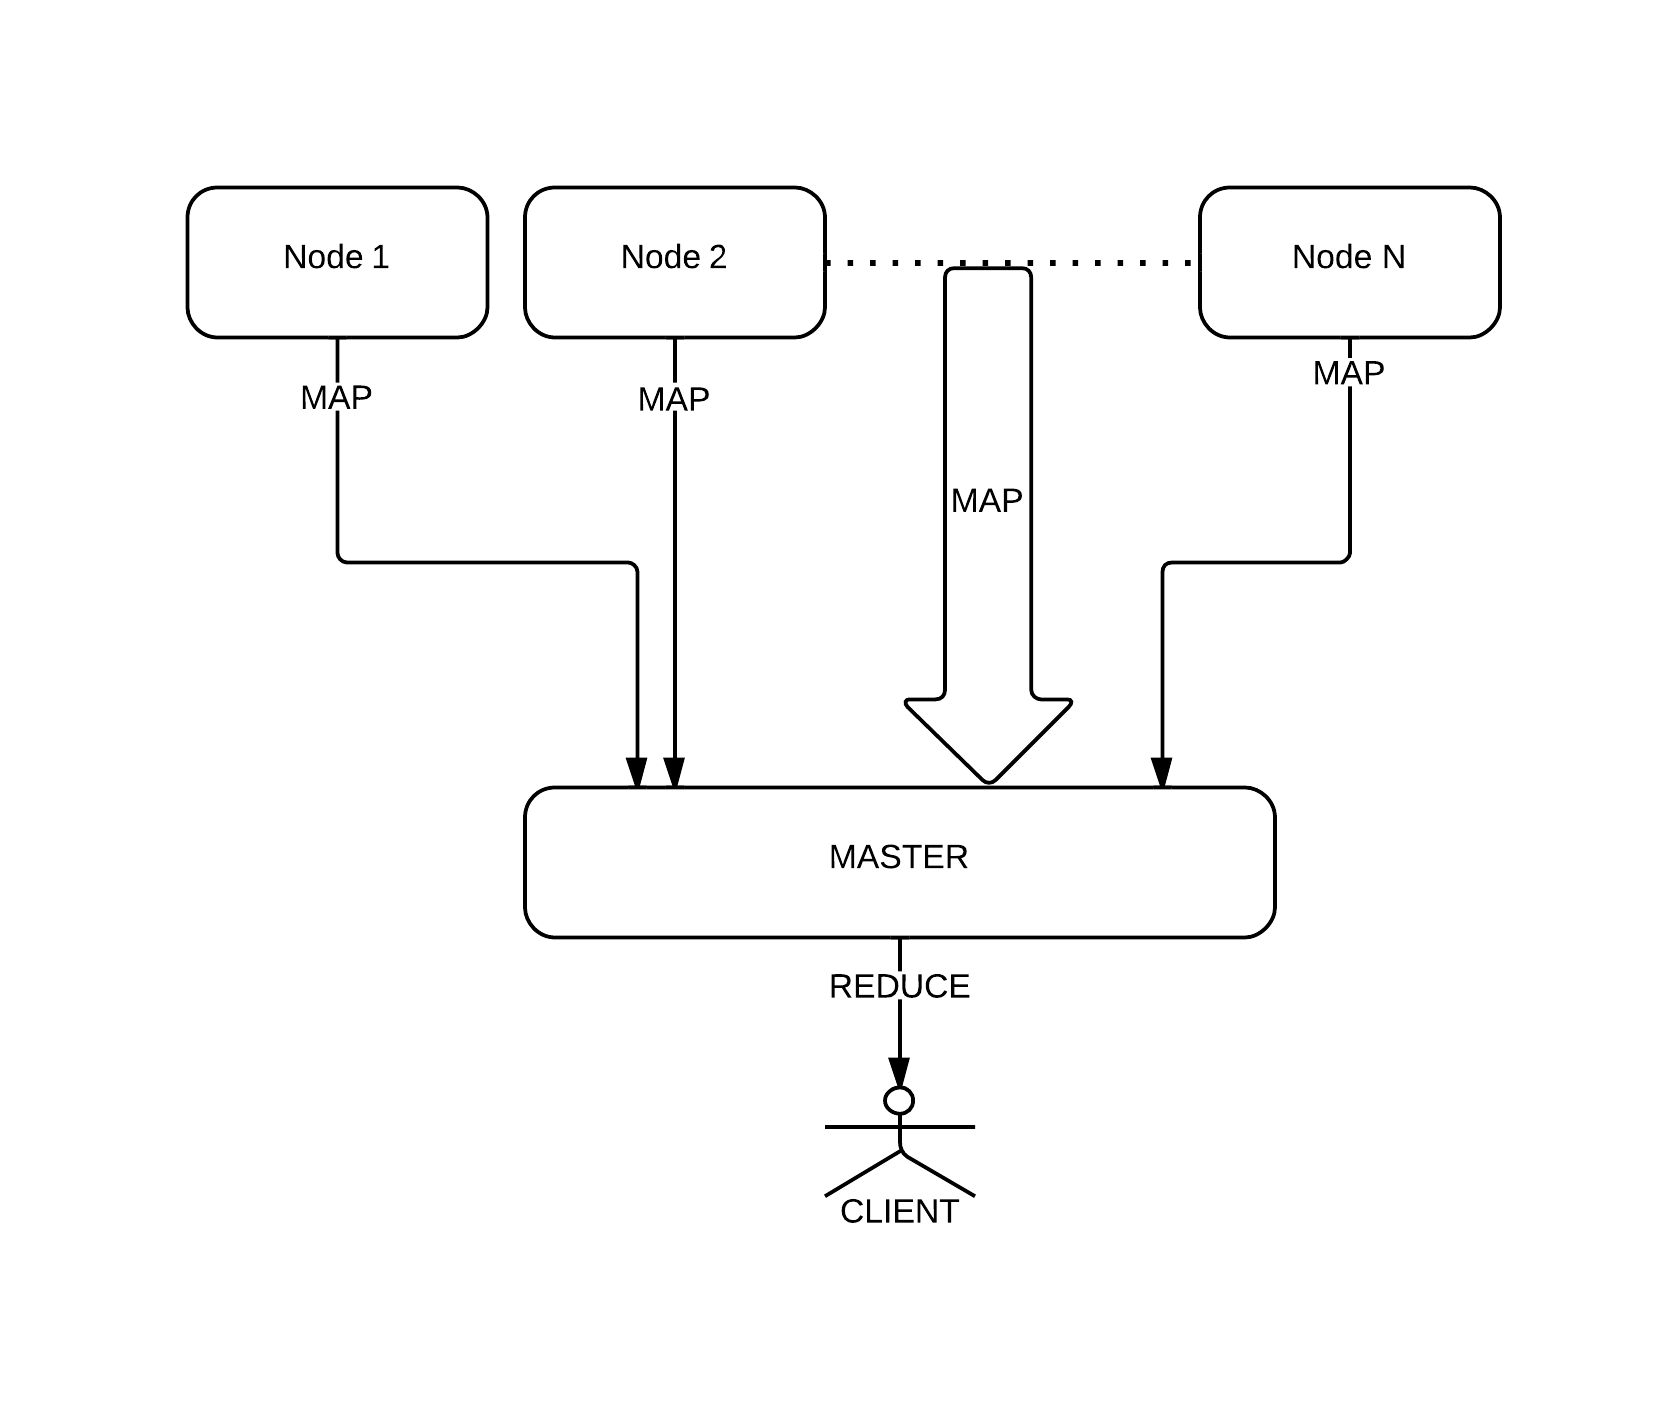
\includegraphics[width=0.9\textwidth, height=0.7\textwidth]{MapReduce}}
			\end{center}
		\end{figure}
	\item Każdy z węzłów poprzez użycie Mappera, który korzystając z wiedzy o położeniu danych w pamięci na karcie graficznej przechowywanej w B+ drzewie filtruje dane tworzy
		pary taskId - record. W ten sposób Mapper wykonuje operację map. Dane te mogą być dodatkowo zagregowane na karcie przez Composer'a. Wykonuje on na zmapowanych
		parach operację Compose - nazywaną przez nas operacją Reduce ponieważ jest ona analogiczna do tej, którą ma wykonać na końcu Master. Tutaj mamy zamiar wykorzystać
		moc obliczeniową kart graficznych. Uzyskane dane z wielu kart graficznych mogą być wstępnie zagregowane już na węźle jeśli pozwala na to rodzaj operacji Reduce - musi być łączna i przemienna.
		\begin{figure}[t]
			\begin{center}
				\caption{Schemat działania Map-Reduce w węźle}
		 		\makebox[\textwidth]{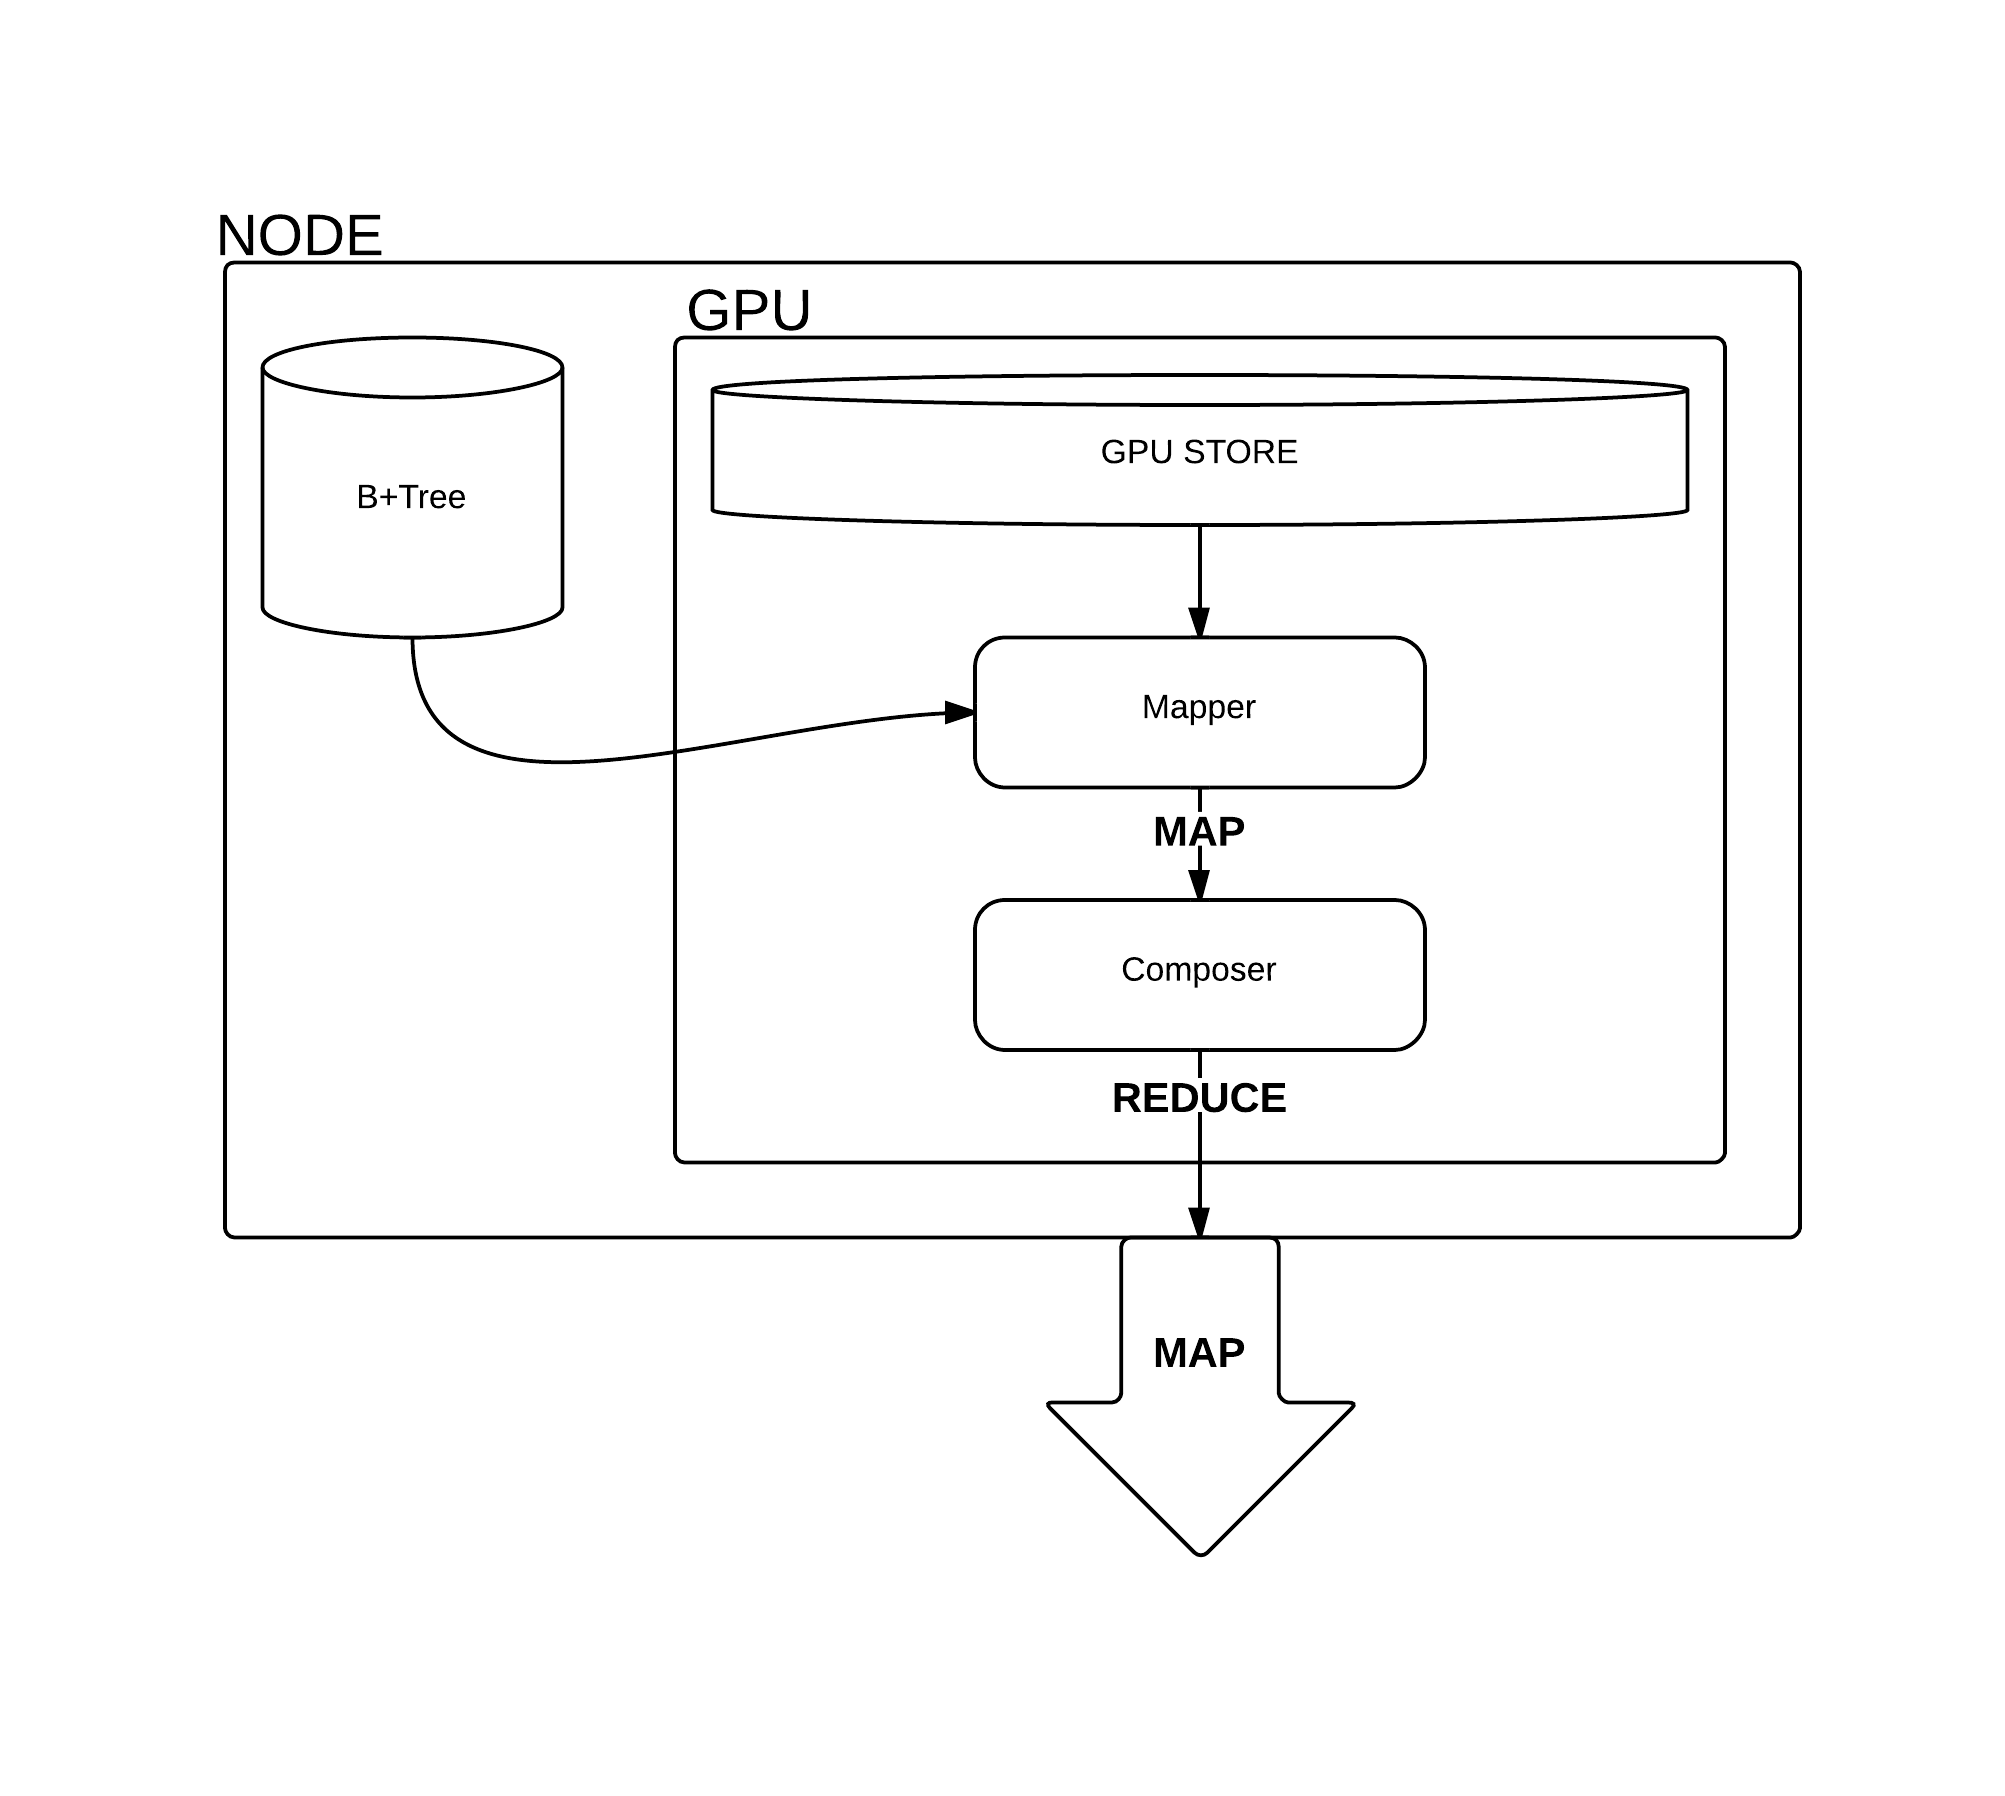
\includegraphics[width=0.9\textwidth, height=0.7\textwidth]{MapReduce_Node}}
			\end{center}
		\end{figure}
\end{itemize}
\clearpage

Taki model systemu może zapewnić dużą skalowalność systemu. W przyszłości operacje Reduce Mastera będą mogły być wykonywane również na zarezerwowanej dla niego karcie graficznej (jeśli okaże się to korzystne).

\section{Pierwszy prototyp programu}
%	\subsection{Opis funkcjonalności}

	\subsection{Przeprowadzone testy}
	Po pierwszym etapie implementacji podjęliśmy pierwszą próbę zmierzenia wydajności systemu. Testy wydajności zostały przeprowadzone za pomocą programu Apache Benchmark. Jako że do tej pory aplikacja była uruchamiana jedynie z użyciem jednej maszyny z jedną karta graficzną, testy zostały przeprowadzone w takim samym środowisku. Testy zostały przeprowadzone po to, by dać nam podstawowe pojęcie o ograniczeniach obecnej implementacji systemu. Testy przeprowadzane po kolejnych etapach implementacji będą ważnym składnikiem oceny wydajności projektu
	
		\subsubsection{Test wydajności umieszczania danych na karcie}
		W tym teście wykonywano $20000$ zapytań typu Insert przez kolejno $1, 2, 3, 4, 5, 6, 7, 8, 10, 15, 30, 40$ wątków klienta. Dane z tego testu przedstawione są na wykresach \ref{fig:concurrency} i \ref{fig:concurrencyPerThread}. 
		\begin{figure}[ht!]
	\centering
	\caption{Liczba zapytań na sekundę}
	\label{fig:concurrency}
		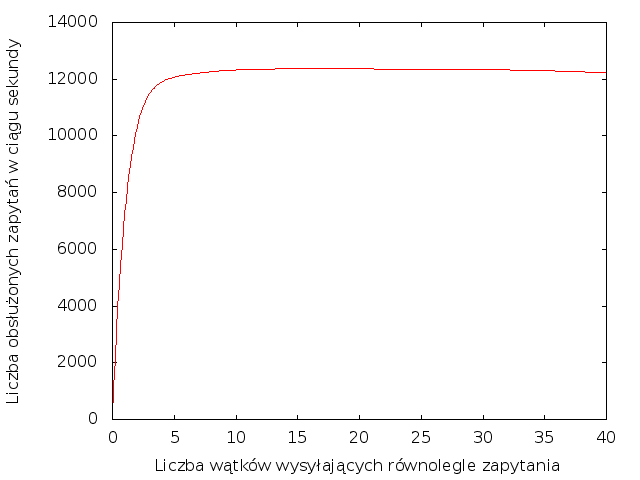
\includegraphics[width=0.8\textwidth]{img/concurrencyTest.png}
	\end{figure}
	
	 
		\begin{figure}[ht!]
	\centering
	\caption{Liczba zapytań na sekundę w przeliczeniu na wątek}
		\label{fig:concurrencyPerThread}
		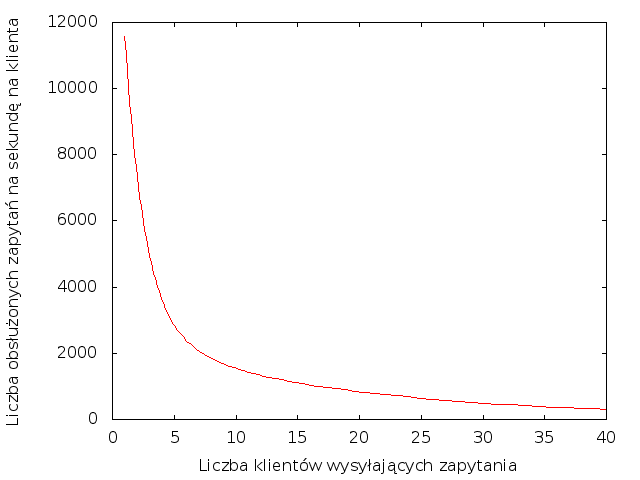
\includegraphics[width=0.8\textwidth]{img/concurrencyTestPerThread.png}
	\end{figure}
	
Rysunek \ref{fig:concurrency} pokazuje, że liczba zapytań obsłużonych w ciągu sekundy przestaje rosnąć, gdy osiągnie wartość ok 12000. Jest to w pewnym przybliżeniu maksymalna liczba zapytań jaką system jest w stanie obsłużyć w ciągu sekundy. Oczywiście należy wziąć pod uwagę, że wyniki mogą różnić się w zależności od mocy sprzętu, na którym uruchamiany jest program. 


Na wykresie \ref{fig:threads} przedstawiony jest wynik testu, w którym wysyłano $100000$ zapytań przez kolejno $1, 20, 50, 100$ wątków klienta. Czas odpowiedzi na zapytania dla każdej serii umieszczono na jednym wykresie. Pokazuje to różnicę w czasie przetwarzania żądania w zależności od liczby równoległych zapytań.

		\begin{figure}[ht!]
	\centering
	\caption{Czas odpowiedzi w zależności od liczby wątków}
		\label{fig:threads}
		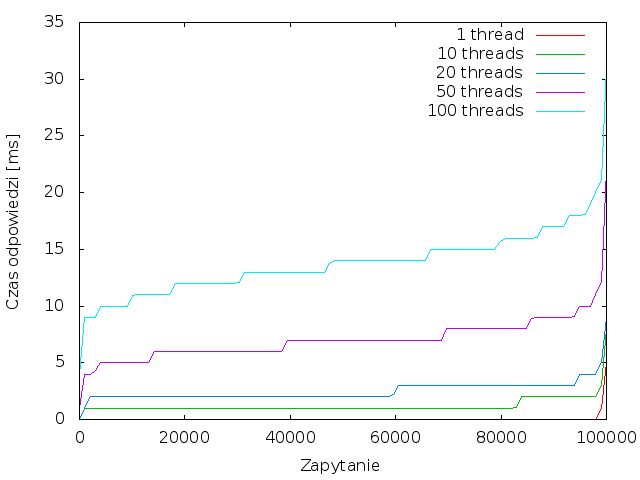
\includegraphics[width=0.9\textwidth]{img/threadsTest.png}
	\end{figure}
	
 

\section{Przyszłość}
W kolejnym etapie prac priorytetem będzie obsługa zapytań select wraz z agregacją danych. Równolegle będziemy prowadzić prace nad uruchomieniem systemu na wielu urządzeniach oraz docelowo na klastrze z wieloma kartami graficznymi tak, aby móc dokładniej przetestować wydajność systemu.
\end{document}